\documentclass[12pt]{paper}
%\usepackage{paper} %if the document does not compile properly for you on the initial build, uncomment \usepackage{paper} and build again. This should force MikTeX to install package "paper"
\usepackage[margin=1in]{geometry}
\usepackage{float}
\usepackage{natbib}
\bibliographystyle{apsr}
\usepackage{graphicx}
\graphicspath{ {../fig/} }
\usepackage{setspace}
\usepackage[super]{nth}
\usepackage{booktabs}
\usepackage{makecell}
\usepackage{amsmath}
\usepackage{dcolumn}
%\usepackage{authblk}
\usepackage{hyperref}
\usepackage{wrapfig}
\usepackage{amsmath}
\usepackage{adjustbox}
\usepackage{hanging}
%\usepackage{etoolbox}
%
%\AtBeginEnvironment{quote}{\singlespacing\small}
\usepackage{epigraph}

\newlength{\cslhangindent}
\setlength{\cslhangindent}{1.5em}
\newenvironment{cslreferences}%
{\setlength{\parindent}{0pt}%
	\everypar{\setlength{\hangindent}{\cslhangindent}}\ignorespaces}%
{\par}

\title{Give a Man a Fish and He'll Eat for a Day, But Will He Vote for You?: Explaining the Political Quiescence of Aid Beneficiaries in the United States}
\author{Sarah R. Warren}
\date{}

\begin{document}
\maketitle

\setlength\epigraphwidth{.8\textwidth}
\epigraph{We do not have a government by the majority. We have a government by the majority who participate.}{\textit{Thomas Jefferson}}
%\thispagestyle{empty}
%\clearpage
%\setstretch{1}

\section*{Introduction}
Voting is the heart of democracy. A vote sends a direct message to the government about how someone wants to be governed. But who is represented and who holds representatives accountable depends entirely on who votes. Groups who fail to turn out in large numbers effectively have a mute in their political voice. In this paper, I examine why a particular group, public aid beneficiaries, often turnout in low numbers, despite an unusually visible stake in election outcomes. Seymour Lipset (1960) argued that one's decision to vote depends upon the perceived “relevance of government policies to the individual.” One might, therefore, expect public aid beneficiaries to be more politically active than other citizens (Olson 1965). Public funding priorities have a direct impact on the quality and quantity of food, healthcare, and spending money these households receive. Yet it is well-established that voters with lower education and income turnout less often than their higher-resourced counterparts (Wolfinger and Rosenstone 1980). Among low income voters, public assistance recipients are an especially quiescent voting bloc (Verba, Schlozman, and Brady 1995). 47\% of eligible adults with family incomes of less than \$20,000 a year voted in 2012 and just 25\% voted in the 2010 midterm elections. As political scientists, how can we reconcile our theoretical predictions with this observed behavior?

In this paper, I build on existing theories of attribution and voter behavior to model an explanation for the voting behavior of American welfare recipients. I use a dynamic Bayesian model with incomplete information to highlight partisanship as a mechanism which can cause variation in turnout among aid recipients. Having done so, I develop hypotheses which will hold if this model is useful as a picture of the world (Rubinstein 1991, 2006; Johnson 2020). I empirically evaluate the implications of my model using data from the Maxwell Poll from 2004-2007. The rest of the paper proceeds as follows. In Sections 1-2, I discuss the dominant theories of the quiescence of aid recipients and discuss the contribution of this paper in the broader literature. In section 3, I present my formal theory of voter behavior and federal redistribution. In Sections 4-5, I present my empirical design and analysis. I conclude in Section 6 with a discussion of my results and directions for future work.

\section{The Quiescence of Aid Recipients}
Voter participation is among the most widely studied components of political behavior. As such, scholars have long considered the individual, social, and systemic factors that influence the decision to turn out on election day. Modern theories of voting behavior still rely on Lipset’s (1960) summation of the boundedly rational political actor: voters turnout based on the perceived relevance of politics to their own lives (Conover, Feldman, and Knight 1986; Conover, Feldman, and Knight 1987; Dowding 2005; Feddersen and Sandroni 2006). Thus, what matters is not simply the objective relevance of government to the voter, but the extent to which government agents can effectively claim credit (or avoid blame) for governmental action that citizens perceive to affect them (Mayhew 1974). Presumably, then, those who stand to benefit the most from generous government policies (and, conversely, be most harmed by social spending cuts) should be likely to vote. What, then, can explain the relative silence of public aid beneficiaries in the United States?

There are two widely accepted reasons for the quiescence of aid-receiving voters in the United States. First, because aid recipients are often less well educated and less well off financially, the boost to their participation by their larger interest in government activity is insufficient to overcome their other resource deficits (Verba, Scholzman, and Brady 1995). The benefits they receive, too, are insufficient to close the resource gap. Second, aid institutions in the United States diminish the perceived self efficacy of aid-recipients, making them less likely to turnout to vote. Previous work highlight the educative effects of institutions, which shape the behavior of aid participants (Madsen 1968; Pateman 1970; Piven and Cloward 1971). Soss (1999) and others (Madsen 1986; Mettler and Soss 2004; Mettler and Stonecash 2008; Chen 2013) argue that institutions like means-testing\footnote{Means-tested aid means simply that recipients must be below a certain level of wealth and income to qualify for these benefits. Universal aid and entitlements do not require an income test.} teach participants that government is not responsive to them. Participants carry this sense of low self efficacy to other political processes, including as voting, leading to decreased turnout.\footnote{Other scholars, however, find that aid intended for the very poor can have a very positive effect on political participation around the world (De La O 2013; Manacorda et al. 2011; Labonne 2013; Pop-Eleches and Pop-Eleches 2012).} Because self efficacy is a latent quality—and can, at best, be observed through self-reported measures—scholars use means-testing as its empirical proxy. In other words, self efficacy is a theoretical prior and is rarely empirically evaluated as the true causal mechanism that decreases voter turnout.

Some models (Fiorina 1981; Kinder and Kiewiet 1981) suggest that voters choose presidential candidates based on their own financial circumstances, via “pocketbook voting.” In these attributive models, voters take stock of factors such as their personal employment, their health benefits, their income, and other changes to their personal financial situation. Based on these, voters either blame the incumbent for their bad circumstances or credit him with their good circumstances. Other models (Goren 1997; Gomez and Wilson 2001) suggest that voters are sociotropic, or base their economic attributions on national economic factors, such as the GDP, the stock market, inflation, and the unemployment rate. In these models, voters retrospectively blame the incumbent president for rising unemployment and inflation, a falling GDP, and rising taxes.  However, economic voters may be heterogeneous in their response to information. Weatherford (1978) finds that pocketbook responses vary by social class. Conover, Feldman, and Knight  (1986) find that voters differ in the quantity and quality of information they have on the national economy and how they apply it. CFK find that the accuracy of retrospective assessments depends jointly on the availability of information about the issue, the salience of the issue, and the sensitivity of the issue to specific knowledge. Similarly, Hansford and Gomez (2015) find that economic evaluations are colored by appraisals of the incumbent and thus do not operate as an exogenous influence on votes. Thus, the decision to vote and for whom to vote as the joint product of the information about the costs and benefits of voting and how that information is processed. Differences in “processing” most often manifest through partisanship, education, or political sophistication (Gomez and Wilson 2001; Arceneaux 2006; Chen 2013). 

These conventional models of voter behavior and motivation speak to the processes which undergird all voter decisions. While parsimonious, however, these theories struggle to account for the unique circumstances of aid beneficiaries. Social welfare (1) may impose a unique set of costs on participants through means-testing, (2) may confer a uniquely salient set of benefits through cash transfers or subsidization, (3) and may mitigate the type and salience of economic information recipients process. My novel theory of aid-related voting behavior addresses these contradictory literatures by proposing a general theory of the effect of aid on voters across the political spectrum. Importantly, the mechanism I highlight in my model is the interaction between aid and partisanship, which I then test empirically.

\section{Reevaluating the self efficacy Hypothesis}
Self efficacy is often credited as the mechanism for the political quiescence of aid beneficiaries in the United States. Soss (1999) and others (Mettler and Stonecash 2008; Chen 2013) argue that means-testing teaches participants that government is not responsive to them and that participants develop low self efficacy. The causal logic here is that being constantly asked to prove how impoverished they are and about the efforts they are making to change their situation leaves participants feeling like they have little agency in their lives. Participants carry over this sense of low efficacy to other political processes, including voting. Because those participating in universal aid programs do not participate in the means-testing feedback loop, it follows that we should not expect this type of aid to decrease the likelihood of voting. Indeed, Mettler and Stonecash (2008) argue that universal aid programs actually increase the probability of turning out to vote.  

As a cursory analysis, I plot the relationship between aid-type and self-efficacy using the Maxwell Poll data from Mettler and Stonecash (2008). The Maxwell Poll asks respondents, ``Do you agree or disagree with this statement: `People like me don’t have much say about what government does'?" Agree is coded as 0, indicating low self efficacy, while disagree is coded as 1, indicating high self efficacy. From the figure, we can see that there is not an obvious relationship between low self efficacy and aid type. While there are more means-tested programs respondents could participate in, generally, respondents appear to report low and high self efficacy with similar frequencies across programs.

%PUT FIG HERE

Previous work dichotomizes aid as either means-tested or universal. However, I argue that this conceptualization of aid is lacking in two important ways. Firstly, entitlements are meaningfully distinct from other forms of universal aid, such as FEMA or Social Security Disability Insurance (SSDI). Beneficiaries are entitled to their benefits because they made a costly effort to obtain them. To be eligible for entitlements, one must put forward a costly effort, either by serving in the United States military (GI Bill) or paying into the program until age 65 (Social Security). Secondly, federally subsidized loans to students and businesses are often categorized as means tested aid, but differ importantly from other forms of means-tested aid because recipients must pay back the loan in the future. Importantly, this kind of government assistance comes at a future cost to the recipient – a cost equal to or greater than the value of the aid. To account for this heterogeneity, I divide aid into four types: universal aid, entitlements, loans, and means-tested aid.

\begin{table}[]
	\begin{adjustbox}{width=1\textwidth}
		\begin{tabular}{llll}
			\hline
			\textbf{Entitlements} & \textbf{Loans} & \textbf{Means-Tested} & \textbf{Universal}                   \\ \hline
			Social Security       & Student Loans  & Food Stamps           & Unemployment                         \\
			Medicare              & Business Loans & Medicaid              & Social Security Disability Insurance \\
			Government Pension    &                & Welfare               & Workers' Comp.                       \\
			Veterans Benefits     &                & EITC                  &                                      \\
			GI Bill               &                & Public Housing        &                                      \\
			&                & WIC                   &                                      \\
			&                & HeadStart             &                                      \\
			&                & College Grant         &                                      \\
			&                & Mortgage Tax Credit   &                                      \\ \hline
		\end{tabular}
	\end{adjustbox}
	\caption{Aid Programs by Type} 
	\label{}
\end{table}



To further evaluate the self efficacy hypothesis, I regress several measures of aid on self-reported self efficacy, testing the association between the aid a person receives and their self-reported self efficacy. The directional results and significance levels are reported in Table 2, but the full table with coefficients can be found in Appendix B.

\begin{table}[!htbp] \centering 
	\begin{adjustbox}{width=1\textwidth}
		\begin{tabular}{@{\extracolsep{5pt}}lD{.}{.}{-3} D{.}{.}{-3} D{.}{.}{-3} D{.}{.}{-3} D{.}{.}{-3} D{.}{.}{-3} D{.}{.}{-3} } 
			\\[-1.8ex]\hline \\[-1.8ex] 
			\\[-1.8ex] & \multicolumn{7}{c}{Self Efficacy} \\ 
			\\[-1.8ex] & \multicolumn{1}{c}{(1)} & \multicolumn{1}{c}{(2)} & \multicolumn{1}{c}{(3)} & \multicolumn{1}{c}{(4)} & \multicolumn{1}{c}{(5)} & \multicolumn{1}{c}{(6)} & \multicolumn{1}{c}{(7)}\\ 
			\hline \\[-1.8ex] 
			Aid Dummy & -^{***} & -^{***} &  &  &  &  &  \\ 
			Total Aid &  &  & -^{**} &  &  &  &  \\ 
			Count: Total Universal Aid &  &  &  & -^{***} &  &  &  \\ 
			Count: Total Loans &  &  &  &  & + &  &  \\ 
			Count: Total Entitlements &  &  &  &  &  & - &  \\ 
			Count: Total Means-Tested &  &  &  &  &  &  & - \\ 
			Republican (dummy) & +^{***} & - & +^{***} & +^{***} & +^{***} & +^{***} & +^{***} \\ 
			Aid Dummy x Republican &  & + &  &  &  &  &  \\ 
			N & \multicolumn{1}{c}{458} & \multicolumn{1}{c}{458} & \multicolumn{1}{c}{458} & \multicolumn{1}{c}{458} & \multicolumn{1}{c}{458} & \multicolumn{1}{c}{458} & \multicolumn{1}{c}{458} \\ 
			Log Likelihood & \multicolumn{1}{c}{-363.801} & \multicolumn{1}{c}{-363.818} & \multicolumn{1}{c}{-366.801} & \multicolumn{1}{c}{-364.065} & \multicolumn{1}{c}{-367.867} & \multicolumn{1}{c}{-368.173} & \multicolumn{1}{c}{-367.896} \\ 
			AIC & \multicolumn{1}{c}{743.602} & \multicolumn{1}{c}{745.636} & \multicolumn{1}{c}{749.603} & \multicolumn{1}{c}{744.131} & \multicolumn{1}{c}{751.735} & \multicolumn{1}{c}{752.346} & \multicolumn{1}{c}{751.793} \\ 
			\hline \\[-1.8ex] 
			\multicolumn{8}{l}{$^{*}$p $<$ .1; $^{**}$p $<$ .05; $^{***}$p $<$ .01} \\
			\multicolumn{8}{c}{\footnotesize Note: All models include controls for sex, education, income, race, following public affairs, and trust in government.} 
		\end{tabular} 
	\end{adjustbox}
	\caption{The Relationship Between Aid and Self Efficacy} 
	\label{}
\end{table} 

Receiving aid is, on average, associated with lower self efficacy and, as the total number of aid programs participated in increased, the likelihood of having high self efficacy decreases. However, in contrast to previous work, I find that as the number of universal aid programs a respondent benefits from increases their likelihood of low self efficacy increases $(p < 0.01)$. No other form of aid has a statistically significant effect on the likelihood of having low self efficacy, though the coefficient on the count of means-tested aid is appropriately signed. Given these results, the evidence for the self efficacy mechanism is murky. If receiving universal aid decreases the likelihood of having high self efficacy, how can low self efficacy be the mechanism by which aid depresses turnout only among voters receiving means-tested aid?

In the following section, I propose a theory of federal aid and voter behavior which does not depend on self efficacy as the mechanism by which aid depresses certain voters' turnout. My theory simply proposes that it is costly to voters to have an Executive who is ideologically distant from them, but that tangible benefits from the Executive can offset these costs. I present the full mathematical model below but give a conceptual overview here. 

Following Gomez and Wilson (2003), voters credit the incumbent President with the distribution (or lack thereof) of aid prior to an election. Gomez and Wilson (2003) demonstrate that, for most voters, the President is the figurehead of the government and is, therefore, the easiest attributive link between federal action and individual opinion. Therefore, while acknowledging that aid is a complex process involving federal, state, and bureaucratic actors, my model includes only the attributive relationship between the Voter (V) and the Incumbent (I). I argue that aid-receiving voters prefer Executives that prioritize aid-spending and especially prefer aid-prioritizing Executives that are in their political party. However, during elections, they cannot know whether the Incumbent is \textit{truly} an aid-prioritizing candidate. The best voters can do is make an educated guess based on the Incumbent's history of redistribution. If the Incumbent has delivered aid in the past, members of his party are motivated to turnout to reelect him. Members of the opposition party, however, are not necessarily more likely to vote for the Incumbent, but they are less motivated to turnout to vote against him.

This theory has two unique advantages over traditional models. First, spatial models of redistribution and voter behavior assume that the mechanism by which aid alters electoral outcomes is by altering vote choice (Cox and McCubbins 1986; Stokes 2005). The long-standing debate on how candidates should distribute targetable goods question pits Cox and McCubbins's (1986) ``core voter model” against Lindbeck and Weibull's (1987) ``swing voter model.” Cox and McCubbins argue that vote-maximizing parties will allocate distributive benefits primarily to their core voters - and not to their opposition. Meanwhile, the swing voter logic holds that ``voters who are predisposed in favor of [a party] on partisan or programmatic grounds [– that is, its core voters –] cannot credibly threaten to punish their favored party if it withholds [distributive] rewards. Therefore the party should not waste rewards on them," (Stokes 2005, 317). Instead, I argue that aid alters electoral outcomes by altering voter turnout. Empirically, this is convenient because, while vote choice is private, data on voter turnout is easily accessible. Further, I also demonstrate that candidates benefit by distributing aid even to their opposition.

In this vein, the second advantage of my model is that my core argument - that partisanship will generally determine vote choice, but factors like redistribution can affect turnout - is supported by a rich body of literature on partisanship and swing voters. It is generally agreed upon that partisanship is an important factor when considering vote choice (Campbell et. al 1960; Achen and Bartels 2016), that "swing" voters are increasingly rare (Bitecofer 2018), and that inter-party polarization is on the rise (Abramowitz 2010; Iyengar et al. 2012; Ahler and Sood 2018). Thus, rather than argue that incumbents can buy their weak opposition with redistribution, I instead argue that they can mobilize their base and depress their opposition.

\section{A Formal Model of Aid and Attribution}
\textbf{Players:} Two politicians, an incumbent (I) and a challenger (C), who have different ideal points $(x_I=1, x_C=0)$. A voter (V) whose ideal point $x_V \epsilon [0,1]$ lies somewhere between $x_I$ and $x_C.$

\textbf{Player Types:} Nature selects the politicians’ types, $\theta_I, \theta_C \epsilon \{0,1\}$, with probabilities: $Pr(\theta_I=0)=Pr(\theta_I=1)=Pr(\theta_C=0)=Pr(\theta_C=1)= \frac{1}{2}$ Nature privately reveals $\theta_I,\theta_C$ to I and C, respectively. Type $\theta=0$ prefers not to deliver aid the voter though delivers aid with some positive probability. Type $\theta=1$ prefers to deliver aid though fails to deliver aid with some positive probability. The probability that the politician delivers aid in accordance with his type is $p > 1 – p$ or $p > \frac{1}{2}$.\footnote{In the real world, politicians have some control over the types of aid they distribute. However, often, the need for aid, and the need for a certain kind of aid, is determined by apolitical circumstances, such as a hurricane, a stock market crash, or a pandemic. Because of this, I make the simplifying assumption that Incumbents' aid preferences are exogenous and that Incumbents do not always behave according to their type to mirror real-world pressures and constraints.}

\textbf{Sequence of Play}
\begin{enumerate}
	\item Nature determines each politician’s type, $\theta_I, \theta_C \epsilon \{0,1\},$ with probabilities $(\frac{1}{2}, \frac{1}{2})$ and reveals types privately to I and C, respectively.
	\item Incumbents pick the first period aid amount, $y_1\epsilon \{0,1\}.$ The incumbent behaves according to his type with greater likelihood than not. First period aid $y_1\epsilon \{0,1\}$ is administered.\footnote{Of course, not all aid is created equally. Some aid programs require impose a great administrative burden on potential beneficiaries in order to qualify. This burden - in the form of extensive employment and medical histories, visits and interviews with case workers, drug tests, etc. - may offset the value of the aid received. I consider this possibility in Appendix A, where I present a conceptual expansion of this model in which the aid delivered in $t_1$ varies continuously between $[0,1]$.}
	\item Nature determines the cost of voting, $c~U[0,1]$ and reveals this cost to voter V.
	\item The voter V chooses whether to vote, $v \epsilon \{0,1\}$
	\item If V votes $(v=1)$, then he decides the election winner, I or C. If V does not vote $(v=0)$, Nature decides the election winner, I or C.
	\item The winner (I or C) picks the second period aid amount, $y_2 \epsilon \{0,1\}$. The winner behaves according to his type with greater likelihood than not. Second period aid  $y_2 \epsilon \{0,1\}$ is administered.
\end{enumerate}

\textbf{Politicians' Utility}: In each period $t \epsilon \{1,2\}$, each politician $p \epsilon \{I,C\}$ receives: 

\begin{gather}
U_{p}^t = -|\theta_p - y_t|
\end{gather}

where $y_t\epsilon \{0,1\}$ is the executive’s choice of distributive aid policy. $\theta_p$ denotes the politician’s type, which represents her preferred distributive policy. Hence, a politician of type $\theta_p = 1$ prefers to deliver aid $(y_t = 1)$, while a politician of type $\theta_p = 0$ always prefers no aid $(y_t = 0).$

\emph{Voter's Utility}: V’s utility function is constant across periods: 
\begin{gather}
U_{V}^t = -|x_o - x_V| + y_t
\end{gather}

where $y_t \epsilon \{0,1\}$ represents the amount of distributive aid awarded to the voter in period $t \epsilon \{1,2\}$, $x_V$ represents the voter’s ideal point, and $x_o$ is the ideal point of the office-holding politician, who is either the Incumbent $(x_I = 1)$ or the Challenger $(x_C = 0).$ Hence, the voter’s utility depends on his ideological proximity to the office holder as well as his benefit from any distributive aid.

In between the two periods, the voter may choose to vote in the election by incurring a turnout cost, $c$, which is randomly drawn by Nature from the uniform distribution $c~U[0,1]$ and revealed to $V$ prior to the election. $V$’s payoff for the entire game is therefore given by:

\begin{gather}
U_{V}^1 + U_{V}^2 - c \times v
\end{gather}

where $v \epsilon \{0,1\}$ is V’s choice of whether to turn out in the election, and $U_{V}^1$ and $U_{V}^2$ are V’s payoffs from the first and second periods, respectively.

\emph{Voter Beliefs}: The Voter V does not observe the politician types, $\theta_I$ and $\theta_C$, that Nature randomly chooses. Instead, V can only observe the Incumbent's first-period distributive policy,  $y_1$, and form updated beliefs about I’s type. Let $p_{\theta_I} (\theta_p | y_1 )$ denote the V’s posterior beliefs about the probability that $\theta_I = 1$ after observing $y_1$.

\subsection{Equilibria}
For simplicity, I assume that Voter V resolves indifference in favor of abstaining.
	
\textbf{Lemma 1:} In each period $t \epsilon \{1,2\}$, the office-holding executive, $p \epsilon \{I,C\}$, chooses the distributive policy: 
\begin{gather}
x_t=\theta_j (1-p)+ \theta_i (p), 
\end{gather}

where $\theta_j$ is the opposite of the office holder’s type. Incumbent types are therefore not fully separating.

\textbf{Lemma 2:}  After observing the Incumbent’s choice of $y_1 \epsilon {0,1}$ during the first period, the Voter V’s updated belief about the Incumbent’s type is: 
\begin{gather}
p_{(\theta_I)}(p(\theta_i ) + (1 - p)(\theta_j ) | y_1 )=y_1(p)
\end{gather}

Given Lemma 2, V expects to receive $E(y_2 | e=I) = p(\theta_i )+(1-p)(\theta_j)$ units of aid in $t=2$ if I is reelected and $E(y_2 |e=C)=E(\theta_C )=\frac{1}{2}$ units of aid if C wins the election.  V’s expected second period payoff from I’s reelection would be: $EU_V (e=I) = -(1 - x_v ) + [p(y_1 ) + (1 - p)(y_1 )]$ whereas his expected second period payoff from C’s election would be: $EU_V (e=C) = - x_V + \frac{1}{2}$. 

Therefore, conditional on turning out, V votes for I iff: 
\begin{gather}
EU_V (e=I) \geq EU_V (e=C) \Rightarrow = -(1 - x_V ) + [p(y_1 ) + (1 - p)(y_{-1} )] \geq - x_V + \frac{1}{2} \Rightarrow \\
x_V \geq -\frac{3 - 2py_1 - 2y_{-1} - 2py_{-1}}{4}
\end{gather}

When $x_V$ is above the threshold, V prefers that the Incumbent win the election, so V’s total expected payoff from voting would be:
\begin{gather}
 EU_V (v=1 | x_V \geq -\frac{3 - 2py_1 - 2y_{-1} - 2py_{-1}}{4} = - (1 - x_V ) + y_1 - c
\end{gather}

When $x_V$ is below the threshold, V prefers that the Challenger win the election, so V’s total expected payoff from voting would be:
\begin{gather}
 EU_V (v=1 | x_V < -\frac{3 - 2py_1 - 2y_{-1} - 2py_{-1}}{4} = -x_V + \frac{1}{2} - c
\end{gather}

V’s total combined expected payoff from not voting is:
\begin{gather}
EU_V (v=0) = \frac{EU_V (e=I)}{2} + \frac{EU_V (e=C)}{2} = \frac{- (1 - x_V ) + y_1}{2} + \frac{-x_V + \frac{1}{2}}{2} = \frac{y_1}{2} - \frac{1}{4}
\end{gather}

Hence, in equilibrium, V turns out to vote iff: $EU_V (v=1) \geq EU_V (v=0) \Rightarrow c \leq \bar{c}$ where:

\begin{equation}
\bar{c} =
\begin{cases}
\frac{-y_1}{2} - x_V + \frac{3}{4} & if x_V < \frac{1}{4}\\    
x_V (2y_1 - 1) + \frac{3}{4}     & if \frac{1}{4} \leq x_V < \frac{3}{4}  \\
\frac{y_1}{2} + x_V - \frac{3}{4}     & if x_V \geq \frac{3}{4}  \\
\end{cases}
\end{equation}

\textbf{Lemma 3:}
Given turning out, V’s vote in the election is:
\begin{equation}
s =
\begin{cases}
I, & if x_V \geq -\frac{3 - 2py_1 - 2y_{-1} - 2py_{-1}}{4} \\    
C,     & otherwise  \\
\end{cases}
\end{equation}
where $y_{-1}$ is the aid amount not delivered in the period (i.e. if $1$ unit of aid was delivered, $y_{-1} = 0$.) This demonstrates the consequence of candidate types not fully separating in equilibrium: it is entirely possible that the Voter could oust an Incumbent of type $\theta_I = 1$ and keep an incumbent of type $\theta_I = 0$ due to a bad signal.\footnote{If the Incumbent's actions were not determined probabalistically, but were instead allowed to vary their aid policy strategically, it follows, then, that Incumbents would deliver the minimum amount of aid necessary to satisfy the Voter's threshold for $x_v > \frac{1}{2}$ and the minimum amount of aid necessary to repress turnout for $x_v < \frac{1}{2}$.}


\textbf{Lemma 4:} Let $Q_(y_1 )(x_V )$ denote the probability of turnout for a voter with ideal point $x_V$ and who receives $y_1 \epsilon \{0,1\}$ of aid during Period 1. V’s turnout choice in the election is:

\begin{equation}
Q_(y_1 )(x_V ) =
\begin{cases}
\frac{-y_1}{2} - x_V + \frac{3}{4} & if x_V < \frac{1}{4}\\    
x_V (2y_1 - 1) + \frac{3}{4}     & if \frac{1}{4} \leq x_V < \frac{3}{4}  \\
\frac{y_1}{2} + x_V - \frac{3}{4}     & if x_V \geq \frac{3}{4}  \\
\end{cases}
\end{equation}


Given this, we can calculate the \emph{change in turnout probability} from receiving one unit of aid in $t_1$. Put differently, the effect of receiving $y_1 = 1$ is:
\begin{equation}
Q_1 (x_V ) - Q_0 (x_V )=
\begin{cases}
\frac{-1}{2} & if x_V < \frac{1}{4}\\    
2x_V - 1 & if \frac{1}{4} \leq x_V < \frac{3}{4}  \\
\frac{1}{2} & if x_V \geq \frac{3}{4}  \\
\end{cases}
\end{equation}

In other words, delivering aid to ideologically distant voters $(x_V < \frac{1}{2})$ strictly decreases their probability of turning out, while delivering aid to ideologically proximate voters $(x_V > \frac{1}{2})$  strictly increases their probability of turning out. Additionally, conditional upon turnout, delivering aid strictly increases the likelihood of voting for the incumbent. The delivery of aid during period one increases V’s expected payoff from having the incumbent reelected relative to the probability that the aid distribution was an informative signal. The increased expected payoff drives my main prediction that the delivery of aid in period one increases a right-wing voter's probability of turnout.

From Lemmas 1, 2, 3, and 4 we know that those who favor the Incumbent \emph{a priori} credit the Incumbent with the positive experience of aid and, therefore, turnout to vote for him or her. Those who do not favor the incumbent \emph{a priori}, rather than change their vote choice, are simply less motivated to turnout to oust the Incumbent. Distant voters, therefore, should be less likely to turnout to vote at all. Put differently, receiving aid in $t_1$ causes a relatively larger increase in a right-wing voter’s turnout probability but a relatively smaller decrease in a left-wing voter’s turnout probability, given $p > \frac{1}{2}$. If my model paints a useful picture of the world, we should expect to observe the following:

\emph{$H_1:$ For a left-wing voter $(x_V < \frac{1}{2})$, receiving distributive aid in period 1 causes a strict decrease in the probability of voter turnout.}

\emph{$H_2$: For a right-wing voter $(x_V > \frac{1}{2})$, receiving distributive aid in period 1 causes a strict increase in the probability of voter turnout.}

\subsection{Expansion}
Of course, not all aid is created equally.Incumbents may deliver aid to constituents in a way that forces potential recipients to incur a cost, such as the means-testing associated with Medicaid, the supplemental nutrition assistance program (SNAP), or temporary aid to needy families (TANF). Even though authorizing states to administer expedited SNAP in a disaster ultimately delivers aid, individuals must still incur the cost of applying for aid and undergoing means testing. Contrastingly, consider COVID-19 individual aid, for which individuals did not have to apply.
To account for these administrative costs, we might allow the value of aid to vary continuously between 0-1 to represent the personal, psychological, and social costs of obtaining aid. When the Incumbent delivers one unit of aid, regardless of his type, we can write this aid amount as $1 – \delta$, where $\delta \epsilon [0,1]$ and represents the cost potential aid recipients must incur to obtain aid. There may be no cost to participants to obtain aid $(\delta = 0)$; alternatively, the cost of obtaining aid may negate any potential benefit $(\delta = 1)$. Thus, the voter’s expected utility is given by $U_{V}^t = -|x_o - x_V| + [y_t - \delta]$ When $(\delta = 0)$, the expanded model is identical to the original. When $(\delta > 0)$, however, $\delta$ impedes the ability of aid to offset the cost of voting for the incumbent. For simplicity, I represent $y_t - \delta$ as  $\lambda_t$. Now, not only is incumbent type determined exogenously, but so is the value of aid.


The politicians’ utility is still given by,

\begin{gather}
U_{p}^t = -|\theta_p - y_t|
\end{gather}

because the Incumbent does not incur the cost associated with aid. That cost is transferred onto the voter.

The voter’s utility in each period is now given by, 
\begin{gather}
U_{V}^t = -|x_o - x_V| + \lambda_t
\end{gather}

Previously, $y_t \epsilon \{0,1\}$ had either no effect $(y_t = 0)$ or a strictly positive effect $(y_t = 1)$ on V's utility. Now, both $x_V$ and $\lambda_t$ vary continuously between 0 and 1. If $\lambda_t < |x_o - x_V|$, aid will not have a positive effect on V’s utility per round. 

Given that aid is delivered, I assume voters expect $\lambda_t$ to remain constant across candidates. That is, while the deliverance of aid (1) or no aid may vary (0) between rounds, administrative costs should remain constant if the Incumbent remains in power. If voters receive aid in $t_1$ at some value $\lambda_t$, they update their beliefs about the Incumbent based on the expected probability of receiving 0 or $\lambda_t$.

I present the full formalized model and its Lemmas in Appendix A. Going forward, I simply discuss its intuition. As $\delta$ increases (or as $\lambda$ decreases), so does aid's effect on turnout and vote choice. Recall in the baseline model that aid has a strictly negative effect on turnout for left-wing voters $(x_V < \frac{1}{2})$ and a strictly positive affect on right-wing voters $(x_V > \frac{1}{2})$. When aid is allowed to vary continuously, this is no longer the case. Now, only aid that is at or above the threshold condition will influence vote or turnout choice. For the left-wing voter, turnout probability is \textit{increasing} as $\delta$ increases. For the right-wing voter, turnout probability is \textit{decreasing} as $\delta$ increases.

$H_3$: For the left-wing voter $(x_V < \frac{1}{2})$, those participating in aid with low administrative costs will be less likely to turnout to vote than those participating in aid with high administrative costs.

$H_4$: For a right-wing voter $(x_V > \frac{1}{2})$, those participating in aid with low administrative costs will be more likely to turnout to vote than those participating in aid with high administrative costs

\section{Research Design}
To test the implications of my model, I use data from the Maxwell Poll on Citizenship and Inequality from Syracuse University, directed by Jeffery Stonecash. The poll includes data on federal aid status, voter behavior, and civic engagement. The poll is nation-wide annual survey and was administered by phone from 2004-2007. The cumulative data file from the surveys contain weights so that the data is nationally representative and each year averages approximately 600 respondents. I conduct my analysis using binary and ordered logit models, but my results are robust to OLS estimation (see Appendix B). My dependent variable is turnout. The Maxwell Poll asks respondents whether they turnout Always (4), Often (3), Sometimes (2), or Not at all (1). I use this ordinal measure of turnout as well as a binary measure in which I code those who respond ``Always" and ``Often" as 1 and those who responded ``Sometimes" and ``Never" as 0.

My primary independent variable is receiving government aid. I employ several measures of aid across different models to account for heterogeneity within aid programs and account for the cumulative effect of aid on voter behavior. First, I use binary variables for each of the nineteen aid programs contained in the Maxwell Poll dataset in which a 1 means the respondent or a member of the respondent’s household receives the benefit and a 0 means no one in the household receives that benefit. Second, I create a binary variable in which 1 means the respondent or a member of the respondent’s household receives any form of government assistance and a 0 means no one in the household receives government aid. Finally, I use counts of the total number of entitlement, means-tested, universal, and subsidized loan aid the household receives to create an aid-category participation measure. A 0 in all four categories would mean the respondent’s household receives no aid, while a 1 in entitlements and a 0 in the other three categories would mean the respondent’s household receives one kind of entitlement benefit, but no other government aid. This allows me to test $H_3$ and $H_4$, since in general loans and means tested aid have a more strenuous application process, while entitlements and universal aid programs are, on average, easier to enroll in.

For Party ID, I use a binary measure in which a 1 is Republican and a 0 is Democrat. I also include a battery of controls, including race, income, education, sex, how closely the person follows public events, their trust in public officials, and their sense of their self efficacy.

I predict that, given aid, democrats and Republicans will turn out at different rates ($H_1$ and $H_2$). Since the incumbent president during the time of the survey is George W. Bush (R), I predict that Republicans who receive aid will be more likely to turnout than Democratic voters who receive aid. Further, I predict that aid that comes at a high cost to participants will diminish the effect of aid on turnout (i.e. Republicans participating in costlier aid programs will be less likely to turnout than Republicans participating in low-cost aid programs on average).

\section{Analysis}


Recall $H1$ and $H2$ assert that receiving aid \textit{and} party ID cause a change in turnout. To test my hypotheses, I use a dummy variable for aid, which takes on a value of 1 if the respondent benefits from any of the federal aid programs asked about in the survey and 0 otherwise. Using this as my primary independent variable, I estimate a model that interacts Party ID and the Aid Dummy. The results of both the binary and ordered logit for both models are shown in Table 5.
%%Model 3: Vote ~ recieves aid dummy**partyID + controls
\begin{table}[!htbp] \centering 
\begin{tabular}{@{\extracolsep{5pt}}lD{.}{.}{-3} D{.}{.}{-3} } 
\\[-1.8ex]\hline \\[-1.8ex] 
\\[-1.8ex] & \multicolumn{1}{c}{Vote Frequency Dummy} & \multicolumn{1}{c}{Vote Frequency} \\ 
\\[-1.8ex] & \multicolumn{1}{c}{Binary Logit} & \multicolumn{1}{c}{Ordered Logit} \\ 
& \multicolumn{1}{c}{} & \multicolumn{1}{c}{} \\ 
\\[-1.8ex] & \multicolumn{1}{c}{(1)} & \multicolumn{1}{c}{(2)}\\ 
\hline \\[-1.8ex] 
Aid Dummy & 2.755^{***} & 1.058^{*} \\ 
& (0.819) & (0.619) \\ 
Republican & 16.727 & 1.323 \\ 
& (819.837) & (0.955) \\ 
Aid Dummy x Republican & -16.630 & -1.362 \\ 
& (819.837) & (0.983) \\ 
Constant & -0.518 &  \\ 
& (1.161) &  \\ 
N & \multicolumn{1}{c}{458} & \multicolumn{1}{c}{480} \\ 
Log Likelihood & \multicolumn{1}{c}{-128.697} &  \\ 
AIC & \multicolumn{1}{c}{277.395} &  \\ 
\hline \\[-1.8ex] 
\multicolumn{3}{l}{$^{*}$p $<$ .1; $^{**}$p $<$ .05; $^{***}$p $<$ .01} \\
\multicolumn{3}{c}{\footnotesize Note: Standard errors are given in parentheses below coefficients. All models include controls for sex, education, income, race, self efficacy, following public affairs, and trust in government.}  
\end{tabular}
\caption{Aid and Party ID} 
\label{}
\end{table} 

The aid dummy and Republican are positively signed, as predicted in $H1$ and $H2$. However, the interaction between the two is neither significant nor signed as expected. The marginal effects of aid for Democrats are positive while they are negative for Republicans. Thus, I fail to find support for $H_1$ and $H_2$ in Model 2. In fact, I find the opposite. Aid-receiving Democrats are more likely to turnout to vote frequently, all else held constant at 0.

I also measure aid continuously as the count of total aid programs in which a person participates. I interact this total aid measure on party ID. As before, the measures of aid and Republican are signed as predicted, but the coefficient on the interaction term is negative. The marginal effect of aid is once again the opposite of what $H_1$ and $H_2$ predict. Again, I do not find support for my hypotheses.

%%Model 9-10 - Total Aid and Total Aid*PID interaction
\begin{table}[!htbp] \centering 
	\begin{adjustbox}{width=1\textwidth}
\begin{tabular}{@{\extracolsep{5pt}}lD{.}{.}{-3} D{.}{.}{-3} D{.}{.}{-3} D{.}{.}{-3} } 
	\\[-1.8ex]\hline \\[-1.8ex] 
	\\[-1.8ex] & \multicolumn{1}{c}{Vote Frequency} & \multicolumn{1}{c}{Vote Frequency Dummy} & \multicolumn{1}{c}{Vote Frequency} & \multicolumn{1}{c}{Vote Frequency Dummy} \\ 
	\\[-1.8ex] & \multicolumn{1}{c}{Ordered Logit} & \multicolumn{1}{c}{Binary Logit} & \multicolumn{1}{c}{Ordered Logit} & \multicolumn{1}{c}{Binary Logit} \\ 
	& \multicolumn{1}{c}{} & \multicolumn{1}{c}{} & \multicolumn{1}{c}{} & \multicolumn{1}{c}{} \\ 
	\\[-1.8ex] & \multicolumn{1}{c}{(1)} & \multicolumn{1}{c}{(2)} & \multicolumn{1}{c}{(3)} & \multicolumn{1}{c}{(4)}\\ 
	\hline \\[-1.8ex] 
	Total Aid & -0.002 & 0.159^{*} & 0.030 & 0.249^{**} \\ 
	& (0.047) & (0.089) & (0.064) & (0.118) \\ 
	Republican (dummy) & 0.028 & 0.338 & 0.264 & 1.061 \\ 
	& (0.211) & (0.387) & (0.392) & (0.697) \\ 
	Total Aid x Republican &  &  & -0.065 & -0.232 \\ 
	&  &  & (0.090) & (0.180) \\ 
	Constant &  & 0.859 &  & 0.763 \\ 
	&  & (1.002) &  & (1.012) \\ 
	N & \multicolumn{1}{c}{480} & \multicolumn{1}{c}{458} & \multicolumn{1}{c}{480} & \multicolumn{1}{c}{458} \\ 
	Log Likelihood &  & \multicolumn{1}{c}{-133.086} &  & \multicolumn{1}{c}{-132.182} \\ 
	AIC &  & \multicolumn{1}{c}{284.171} &  & \multicolumn{1}{c}{284.363} \\ 
	\hline \\[-1.8ex] 
	\multicolumn{5}{l}{$^{*}$p $<$ .1; $^{**}$p $<$ .05; $^{***}$p $<$ .01} \\
	\multicolumn{5}{c}{\footnotesize Note: Standard errors are given in parentheses below coefficients. All models include controls for sex, education, income, race, self efficacy, following public affairs, and trust in government.}  
		\end{tabular} 
	\end{adjustbox}
\caption{Total Aid} 
\label{}
\end{table} 

If my model usefully reflects the world we live in, those who favor the incumbent \textit{a priori} should be more likely to credit the incumbent with the positive experience of aid and, therefore, turnout to vote for him or her. Those who do not favor the incumbent \textit{a priori} may credit the incumbent with the positive experience of aid, but be unwilling to vote for a candidate from a party they do not prefer. Voters engaging in this attributive process, therefore, should be less likely to turnout to vote at all. Across empirical tests, however, these predictions do not hold. In 2004-2007, receiving aid and being Republican are generally associated with higher turnout, but aid-receiving Republicans have a lower estimated likelihood of turnout than Republicans receiving no aid or aid-receiving Democrats.

This may be due to differences in the costs different aid programs impose on their participants. Some aid programs require detailed income and wealth information, medical and employment histories, monthly interviews, and quarterly reevaluation of eligibility. The costs these programs impose on beneficiaries may diminish the effect of aid on turnout ($H_3$ and $H_4$). In general, government loan programs and means-tested programs impose the highest costs on participants. Entitlements and universal aid programs tend to be easier, on average, for potential beneficiaries to apply for.

In Table 6, I use counts of each of the four types of aid programs as my dependent variables. I predicted that high-cost aid programs, like loans and means-tested aid, would decrease turnout among Republicans and increase aid among Democrats, and that low-cost aid programs, like universal aid and entitlements, would increase turnout among Republicans and decrease aid among Democrats. I find the opposite to be true. Receiving more entitlements are associated with an increase in turnout likelihood in Democrats and associated with a decrease in turnout likelihood among Republicans.

\begin{table}[!htbp] \centering 
	\begin{adjustbox}{width=1\textwidth}
\begin{tabular}{@{\extracolsep{5pt}}lD{.}{.}{-3} D{.}{.}{-3} D{.}{.}{-3} D{.}{.}{-3} D{.}{.}{-3} } 
	\\[-1.8ex]\hline \\[-1.8ex] 
	\\[-1.8ex] & \multicolumn{5}{c}{Vote Frequency Dummy} \\ 
	\\[-1.8ex] & \multicolumn{1}{c}{(1)} & \multicolumn{1}{c}{(2)} & \multicolumn{1}{c}{(3)} & \multicolumn{1}{c}{(4)} & \multicolumn{1}{c}{(5)}\\ 
	\hline \\[-1.8ex] 
	Total Loans & 0.766^{*} & 0.387 &  &  &  \\ 
	& (0.444) & (0.478) &  &  &  \\ 
	Total Universal Aid & 0.492 &  &  & 0.456 &  \\ 
	& (0.342) &  &  & (0.379) &  \\ 
	Total Entitlements & 0.326 &  & 1.702^{**} &  &  \\ 
	& (0.234) &  & (0.739) &  &  \\ 
	Total Means-Tested Aid & -0.089 &  &  &  & 0.048 \\ 
	& (0.145) &  &  &  & (0.148) \\ 
	Republican & 0.288 & 0.125 & 0.902^{**} & 0.238 & 0.310 \\ 
	& (0.393) & (0.427) & (0.453) & (0.446) & (0.514) \\ 
	Total Loans x Republican &  & 0.978 &  &  &  \\ 
	&  & (0.927) &  &  &  \\ 
	Total Entitlements x Republican &  &  & -1.939^{**} &  &  \\ 
	&  &  & (0.788) &  &  \\ 
	Total Universal Aid x Republican &  &  &  & 0.244 &  \\ 
	&  &  &  & (0.676) &  \\ 
	Total Means-Tested Aid x Republican &  &  &  &  & 0.036 \\ 
	&  &  &  &  & (0.289) \\ 
	Constant & 0.790 & 1.332 & 1.173 & 1.339 & 1.346 \\ 
	& (1.049) & (0.968) & (1.009) & (0.962) & (0.981) \\ 
	N & \multicolumn{1}{c}{458} & \multicolumn{1}{c}{458} & \multicolumn{1}{c}{458} & \multicolumn{1}{c}{458} & \multicolumn{1}{c}{458} \\ 
	Log Likelihood & \multicolumn{1}{c}{-130.858} & \multicolumn{1}{c}{-132.550} & \multicolumn{1}{c}{-125.237} & \multicolumn{1}{c}{-132.572} & \multicolumn{1}{c}{-134.406} \\ 
	AIC & \multicolumn{1}{c}{285.715} & \multicolumn{1}{c}{285.100} & \multicolumn{1}{c}{270.474} & \multicolumn{1}{c}{285.145} & \multicolumn{1}{c}{288.811} \\ 
	\hline \\[-1.8ex] 
	\multicolumn{6}{l}{$^{*}$p $<$ .1; $^{**}$p $<$ .05; $^{***}$p $<$ .01} \\
	\multicolumn{6}{c}{\footnotesize Note: Standard errors are given in parentheses below coefficients. All models include controls for sex, education, income, race, self efficacy, following public affairs, and trust in government.}   
		\end{tabular} 
\end{adjustbox}
\caption{Count of Types of Aid} 
\label{}
\end{table} 

\section{Discussion}
Why do aid-receiving voters turn out at such low rates? In this paper, I examine the existing literature and highlight problems with self efficacy, the dominant theoretical mechanism in the literature. I find that it does not conform to theoretical predictions. Then, I present a plausible state of the world in which the effects of aid vary according to political party. I consider the possibility that obtaining aid can be costly and conclude that only low cost programs will have positive (negative) effects for in-party (out-party) voter turnout and vote choice. To evaluate the usefulness of my model, I used data from the Maxwell Poll 2004-2007 to test the hypothesis that aid-receiving Republicans will be more likely to turnout on average than aid-receiving Democrats. In all of my models, I fail to find support for my hypotheses and to reject the null. I also test the effect of aid-type on voter turnout. Counterintuitively, I find that Republicans receiving entitlements are less likely to turnout than Republicans who receive less entitlements, on average.

My work also has three important implications for future work. First, future work would benefit from more suitable data to reevaluate my hypotheses. There is a great need for detailed, individual-level data on aid that is presently only available via a lengthy Freedom of Information Act (FOIA) request process. 

Secondly, future work should consider new ways to reevaluate and measure the self efficacy hypothesis, as my work suggests that it is less straightforward of a mechanism than we believed. 

Thirdly, future work would benefit from further expansions of this theoretical model.
%\bibliographystyle{APSR}
%\bibliography{references.bib}

\clearpage

\section*{Works Cited}
\singlespace 
\begin{hangparas}{.25in}{1}
	
Arceneaux, Kevin. 2006. ‘‘The Federal Face of Voting: Are Elected Officials Held Accountable for the Functions Relevant to Their Office?’’ Political Psychology 27 (5): 731–54.


Baicker, Katherine and Amy Finkelstein. 2019. "The Impact of Medicaid Expansion on Voter Participation: Evidence from the Oregon Health Insurance Experiment," Quarterly Journal of Political Science, vol 14(4): 383-400.


Black, Duncan. 1948. "On the Rationale of Group Decision-making". Journal of Political Economy. 56: 23–34.


Campbell, Angus, Philip Converse, Warren Miller, and Donald Stokes. 1960. The American Voter. New York: John Wiley \& Sons, Inc.
Chen, Jowei. 2013. “Voter Partisanship and the Effect of Distributive Spending on Political Participation.” American Journal of Political Science, 57(1), 200-217.


Conover, Pamela Johnston, Stanley Feldman, and Kathleen Knight. 1986. "Judging Inflation and Unemployment: The Origins of Retrospective Evaluations." The Journal of Politics 48, no. 3 (1986): 565-88


Dowding, Keith. 2005. “Is it rational to vote? Five types of answer and a suggestion.” British Journal of Politics and International Relations. 7:442–459.


Downs, Anthony. 1957. An Economic Theory of Democracy. Harper Collins.


Feddersen, Timothy and Alvaro Sandroni. 2006. "A theory of participation in elections." American Economic Review, 96 (4): 1271-82


Gomez, Brad T. and J. Matthew Wilson. 2001. “Political sophistication and economic voting in the American electorate: A theory of heterogeneous attribution.” American Journal of Political Science 45:899-914.


Hansford, Thomas and Brad Gomez. 2015. “Reevaluating the Sociotropic Economic Voting Hypothesis.” Electoral Studies. 39(10).


Hotelling, Harold. 1929. "Stability in Competition". The Economic Journal. 39 (153): 41–57.


Iyengar, Shanto. 1994. Is Anyone Responsible? How Television Frames Political Issues. Chicago, IL: University of Chicago Press.


Key, V.O. 1966. The Responsible Electorate. Cambridge, MA: Harvard University Press.


Labonne, Julien. 2013. “The Local Electoral Impacts of Conditional Cash Transfers: Evidence from a Field Experiment.” Journal of Development Economics 104 (September): 73–88.


Lipset, Seymour Martin. 1960. Political Man: The Social Bases of Politics. New York. 


Madsen, Douglas. 1987. “Political self efficacy Tested.” American Political Science Review. 81(2): 571–81. doi: 10.2307/1961970.


Manacorda, Marco, Edward Miguel, and Andrea Vigorito. 2011. “Government Transfers and Political Support.” American Economic Journal: Applied Economics 3 (3): 1–28.


Mettler, Suzanne, and Jeffrey Stonecash. 2008. “Government Program Usage and Political Voice.” Social Science Quarterly. 89. 273-293. 


Pateman, Carole. 1970. Participation and Democratic Theory. Cambridge, MA: Cambridge University Press.


Piven, Frances Fox, and Richard A. Cloward. 1971. Regulating the Poor. New York: Vintage Books.


Pop-Eleches, Cristian, and Grigore Pop-Eleches. 2012. “Targeted Government Spending and Political Preferences.” Quarterly Journal of Political Science 7 (3): 285–320.


O, Ana L. De La. 2013. “Do Conditional Cash Transfers Affect Electoral Behavior? Evidence from a Randomized Experiment in Mexico.” American Journal of Political Science 57 (1): 1–14.


Olson, Mancur. 1965. The Logic of Collective Action. Cambridge, MA: Harvard University Press


Riker, William and Peter Ordeshook. 1968. “A Theory of the Calculus of Voting.” American Political Science Review. 62(1): 25-42.


Soss, Joe. 1999. “Lessons of Welfare: Policy Design, Political Learning, and Political Action.” The American Political Science Review, 93(2), 363-380.
Stokes, Susan C. 2005. “Perverse Accountability: A Formal Model of Machine Politics with Evidence from Argentina.” American Political Science Review 99(3): 315–25.


Verba, Sidney, Kay Lehman Schlozman, and Henry E. Brady. 1995. Voice and Equality: Civic Voluntarism in American Politics. Cambridge, MA: Harvard University Press.
U.S. Census Bureau. 2012. “Voting and Registration in the Election of November 2012 - Detailed Tables.” Census.gov. Retrieved: 11/10/2020.
\end{hangparas}
\clearpage


\section*{Appendix A}
\textbf{Voter Beliefs}: The Voter V does not observe the politician types, $\theta_I$ and $\theta_C$, that Nature randomly chooses. Instead, V can only observe the Incumbent's first-period distributive policy,  $\lambda_1$, and form updated beliefs about I’s type.  For the Voter to update, I assume voters treat $\lambda_1 > 0$ as evidence that $\theta_I = 1$. Thus, $p_{\theta_I} (\theta_p | \lambda_1 )$ denote the V’s posterior beliefs about the probability that $\theta_I = 1$ after observing $\lambda_1$. This is because observing any nonzero unit of aid suggests an Incumbent of Type 1, but recall that $\lambda = 1 - \delta$. If $\delta$ is sufficiently high, the Voter will not receive the signal that the Incumbent has delivered aid.

Incumbent types remain probabalistically separating in equilibrium.

V expects to receive $E(\lambda_2 | e=I) = p(\lambda_i) + (1-p)(\lambda_j)$ units of aid in $t_2$ if the Incumbent is reelected. This is because I assume that administrative barriers are constant under the Incumbent. That is, if V received $\lambda_1 > 0$ in $t_1$, he anticipates receiving either $0$ or $\lambda_1$ in $t_2$, but not some other value of $\lambda$ because $\delta_I$ is fixed for the Incumbent.

If, however, C wins the election, Nature draws a new cost of aid, $\delta_C \epsilon [0,1]$. Thus, V expects to receive $E(\lambda_2 | e=C) = E(\theta_C) = \frac{1}{2}$ units of aid if C wins the election.

V’s expected second period payoff from I’s reelection is: 
\begin{gather}
EU_v(e = I) = -(1 - x_V) + [p(\lambda_i) + (1-p)\lambda_j] 
\end{gather}

Whereas his expected payoff from C's reelection is:
\begin{gather}
EU_v(e = C) = -x_V + \frac{1}{2}
\end{gather}

Conditional on turning out, $x_V$ votes for I iff:

\begin{gather}
EU_v(e = I) \geq EU_v(e = C) \rightarrow -(1 - x_V) + [p(\lambda_i) + (1-p)\lambda_j] \geq -x_V + \frac{1}{2} \rightarrow
\lambda_i \geq \frac{3 - 4x_V - 2\lambda_j + 2p\lambda_j}{2p}
\end{gather}

When $x_V$ is above the threshold, the Voter prefers the Incumbent win the election. V's total expected payoff from voting is:
\begin{gather}
EU_v(v = 1 | \lambda_i \geq \frac{3 - 4x_V - 2\lambda_j + 2p\lambda_j}{2p}) = -(1 - x_V) + \lambda_1 - c
\end{gather}

When $x_V$ is below the threshold, the Voter prefers the Challenger win the election. V's total expected payoff from voting is:
\begin{gather}
EU_v(v = 1 | \lambda_i < \frac{3 - 4x_V - 2\lambda_j + 2p\lambda_j}{2p}) = -x_V + \frac{1}{2} - c
\end{gather}

The total expected payoff of not voting is,
\begin{gather}
EU_V (v=0) = \frac{EU_V (e=I)}{2} + \frac{EU_V (e=C)}{2} + \frac{- (1 - x_V ) + \lambda_1}{2} + \frac{-x_V + \frac{1}{2}}{2} = \frac{\lambda_1}{2} - \frac{1}{4}
\end{gather}


\section*{Appendix B}
\subsection{OLS Models}

%%Model 2: Vote ~ all programs + controls (race, income, education, sex, followpa, trustoff, peopsay)
\newgeometry{left=3cm,bottom=0.5cm,right=3cm,top=0.5cm}
\begin{table}[!htbp] \centering 
	\small
	\begin{adjustbox}{width=.6\textwidth}
		\begin{tabular}{@{\extracolsep{5pt}}lD{.}{.}{-3} D{.}{.}{-3} } 
			\\[-1.8ex]\hline \\[-1.8ex] 
			\\[-1.8ex] & \multicolumn{1}{c}{Vote Frequency Dummy} & \multicolumn{1}{c}{Vote Frequency (1-4)} \\ 
			\\[-1.8ex] & \multicolumn{1}{c}{Binary Logit} & \multicolumn{1}{c}{Ordered Logit} \\ 
			\\[-1.8ex] & \multicolumn{1}{c}{(1)} & \multicolumn{1}{c}{(2)}\\ 
			\hline \\[-1.8ex] 
			Republican (dummy) & 0.499 & 0.036 \\ 
			& (0.492) & (0.228) \\ 
			White (dummy) & 0.092 & 0.100 \\ 
			& (0.550) & (0.269) \\ 
			Education & -0.104 & 0.011 \\ 
			& (0.233) & (0.113) \\ 
			Female (dummy) & -0.143 & -0.018 \\ 
			& (0.454) & (0.232) \\ 
			Follow Public Affaris & -0.992^{***} & -0.814^{***} \\ 
			& (0.240) & (0.127) \\ 
			Trust of Government & 1.570^{***} & 0.397^{*} \\ 
			& (0.469) & (0.225) \\ 
			self efficacy & 1.333^{***} & 0.106 \\ 
			& (0.482) & (0.236) \\ 
			Food Stamps & -1.084 & 0.176 \\ 
			& (0.945) & (0.572) \\ 
			Social Security & 4.143^{***} & 0.499 \\ 
			& (1.522) & (0.497) \\ 
			Medicaid & -1.519^{*} & -0.623 \\ 
			& (0.889) & (0.471) \\ 
			Medicare & -2.591^{**} & -0.387 \\ 
			& (1.231) & (0.539) \\ 
			Welfare & -0.599 & -0.038 \\ 
			& (0.971) & (0.531) \\ 
			EITC & -0.292 & -0.496^{**} \\ 
			& (0.514) & (0.245) \\ 
			Unemployment & 1.137^{*} & 0.205 \\ 
			& (0.637) & (0.261) \\ 
			Government Pension & 1.805 & 0.886 \\ 
			& (1.470) & (0.567) \\ 
			Public Housing & 24.027 & 1.310 \\ 
			& (990.845) & (0.909) \\ 
			Disability & 2.172 & 1.374^{**} \\ 
			& (1.468) & (0.664) \\ 
			WIC & 0.249 & -0.345 \\ 
			& (0.770) & (0.385) \\ 
			HeadStart & -2.489^{***} & -1.015^{**} \\ 
			& (0.753) & (0.487) \\ 
			College Grant & 0.455 & 0.089 \\ 
			& (0.634) & (0.292) \\ 
			Student Loans & 0.366 & -0.209 \\ 
			& (0.630) & (0.283) \\ 
			Veterans Benefits & -1.826 & -0.444 \\ 
			& (1.124) & (0.494) \\ 
			Workers' Comp & -0.828 & -0.431 \\ 
			& (0.609) & (0.326) \\ 
			Business Loan & 17.354 & -0.136 \\ 
			& (1,622.703) & (0.571) \\ 
			GI Bill & 0.945 & 0.260 \\ 
			& (1.261) & (0.493) \\ 
			Mortgage Tax Credit & 1.178^{**} & 0.306 \\ 
			& (0.548) & (0.232) \\ 
			Constant & 0.837 &  \\ 
			& (1.214) &  \\ 
			N & \multicolumn{1}{c}{458} & \multicolumn{1}{c}{480} \\ 
			Log Likelihood & \multicolumn{1}{c}{-99.132} &  \\ 
			AIC & \multicolumn{1}{c}{252.264} &  \\ 
			\hline 
			\hline \\[-1.8ex] 
			\textit{Note:}  & \multicolumn{2}{r}{$^{*}$p$<$0.1; $^{**}$p$<$0.05; $^{***}$p$<$0.01} \\
		\end{tabular}
	\end{adjustbox}
	\caption{Program Dummy Variables} 
	\label{}
\end{table}
\restoregeometry


\begin{table}[!htbp] \centering 
	\begin{adjustbox}{width=1\textwidth}
		\begin{tabular}{@{\extracolsep{5pt}}lD{.}{.}{-3} D{.}{.}{-3} D{.}{.}{-3} D{.}{.}{-3} D{.}{.}{-3} D{.}{.}{-3} D{.}{.}{-3} } 
			\\[-1.8ex]\hline \\[-1.8ex] 
			\\[-1.8ex] & \multicolumn{7}{c}{Self Efficacy} \\ 
			\\[-1.8ex] & \multicolumn{1}{c}{(1)} & \multicolumn{1}{c}{(2)} & \multicolumn{1}{c}{(3)} & \multicolumn{1}{c}{(4)} & \multicolumn{1}{c}{(5)} & \multicolumn{1}{c}{(6)} & \multicolumn{1}{c}{(7)}\\ 
			\hline \\[-1.8ex] 
			Aid Dummy & -1.875^{***} & -2.307^{***} &  &  &  &  &  \\ 
			& (0.691) & (0.885) &  &  &  &  &  \\ 
			Total Aid &  &  & -0.090^{**} &  &  &  &  \\ 
			&  &  & (0.045) &  &  &  &  \\ 
			Count: Total Universal Aid &  &  &  & -0.427^{***} &  &  &  \\ 
			&  &  &  & (0.144) &  &  &  \\ 
			Count: Total Loans &  &  &  &  & 0.257 &  &  \\ 
			&  &  &  &  & (0.214) &  &  \\ 
			Count: Total Entitlements &  &  &  &  &  & -0.081 &  \\ 
			&  &  &  &  &  & (0.097) &  \\ 
			Count: Total Means-Tested &  &  &  &  &  &  & -0.112 \\ 
			&  &  &  &  &  &  & (0.072) \\ 
			Republican (dummy) & 0.678^{***} & -0.540 & 0.700^{***} & 0.718^{***} & 0.683^{***} & 0.699^{***} & 0.673^{***} \\ 
			& (0.207) & (1.302) & (0.206) & (0.208) & (0.205) & (0.206) & (0.206) \\ 
			Aid Dummy x Republican &  & 1.250 &  &  &  &  &  \\ 
			&  & (1.322) &  &  &  &  &  \\ 
			Constant & 2.697^{***} & 3.052^{***} & 1.307^{**} & 1.098^{**} & 0.859 & 1.066^{*} & 1.162^{**} \\ 
			& (0.844) & (0.980) & (0.568) & (0.543) & (0.544) & (0.552) & (0.555) \\ 
			N & \multicolumn{1}{c}{458} & \multicolumn{1}{c}{458} & \multicolumn{1}{c}{458} & \multicolumn{1}{c}{458} & \multicolumn{1}{c}{458} & \multicolumn{1}{c}{458} & \multicolumn{1}{c}{458} \\ 
			Log Likelihood & \multicolumn{1}{c}{-363.801} & \multicolumn{1}{c}{-363.818} & \multicolumn{1}{c}{-366.801} & \multicolumn{1}{c}{-364.065} & \multicolumn{1}{c}{-367.867} & \multicolumn{1}{c}{-368.173} & \multicolumn{1}{c}{-367.896} \\ 
			AIC & \multicolumn{1}{c}{743.602} & \multicolumn{1}{c}{745.636} & \multicolumn{1}{c}{749.603} & \multicolumn{1}{c}{744.131} & \multicolumn{1}{c}{751.735} & \multicolumn{1}{c}{752.346} & \multicolumn{1}{c}{751.793} \\ 
			\hline \\[-1.8ex] 
			\multicolumn{8}{l}{$^{*}$p $<$ .1; $^{**}$p $<$ .05; $^{***}$p $<$ .01} \\ 
		\end{tabular} 
	\end{adjustbox}
	\caption{The Relationship Between Aid and Self Efficacy} 
	\label{}
\end{table} 

\begin{table}[!htbp] \centering 
	\caption{Weighted Models 1-3} 
	\label{} 
	\begin{tabular}{@{\extracolsep{5pt}}lD{.}{.}{-3} } 
		\\[-1.8ex]\hline \\[-1.8ex] 
		\\[-1.8ex] & \multicolumn{1}{c}{VOTE} \\ 
		\hline \\[-1.8ex] 
		aid\_dummy & 0.522^{**} \\ 
		& (0.221) \\ 
		PTYIDd & 0.603^{*} \\ 
		& (0.365) \\ 
		white & -0.009 \\ 
		& (0.078) \\ 
		EDUC & -0.008 \\ 
		& (0.030) \\ 
		sex & -0.067 \\ 
		& (0.064) \\ 
		FOLLOWPA & -0.244^{***} \\ 
		& (0.039) \\ 
		TRUSTOFF & 0.105 \\ 
		& (0.064) \\ 
		PEOPSAY & 0.107 \\ 
		& (0.066) \\ 
		aid\_dummy:PTYIDd & -0.623^{*} \\ 
		& (0.372) \\ 
		Constant & 3.301^{***} \\ 
		& (0.266) \\ 
		N & \multicolumn{1}{c}{458} \\ 
		R$^{2}$ & \multicolumn{1}{c}{0.131} \\ 
		Adjusted R$^{2}$ & \multicolumn{1}{c}{0.114} \\ 
		Residual Std. Error & \multicolumn{1}{c}{0.670 (df = 448)} \\ 
		F Statistic & \multicolumn{1}{c}{7.516$^{***}$ (df = 9; 448)} \\ 
		\hline \\[-1.8ex] 
		\multicolumn{2}{l}{$^{*}$p $<$ .1; $^{**}$p $<$ .05; $^{***}$p $<$ .01} \\ 
\end{tabular}
\caption{OLS - Aid Dummy} 
\label{Appendix A.2}
\end{table}


\begin{table}[!htbp] \centering 
	\caption{test} 
	\label{} 
	\begin{tabular}{@{\extracolsep{5pt}}lD{.}{.}{-3} D{.}{.}{-3} } 
		\\[-1.8ex]\hline \\[-1.8ex] 
		\\[-1.8ex] & \multicolumn{2}{c}{VOTE} \\ 
		\\[-1.8ex] & \multicolumn{1}{c}{(1)} & \multicolumn{1}{c}{(2)}\\ 
		\hline \\[-1.8ex] 
		Total & 0.007 & 0.013 \\ 
		& (0.014) & (0.019) \\ 
		PTYIDd & -0.0004 & 0.051 \\ 
		& (0.065) & (0.122) \\ 
		white & 0.023 & 0.019 \\ 
		& (0.075) & (0.076) \\ 
		EDUC & -0.001 & -0.002 \\ 
		& (0.030) & (0.030) \\ 
		sex & -0.051 & -0.055 \\ 
		& (0.064) & (0.064) \\ 
		FOLLOWPA & -0.252^{***} & -0.253^{***} \\ 
		& (0.038) & (0.038) \\ 
		TRUSTOFF & 0.117^{*} & 0.115^{*} \\ 
		& (0.064) & (0.064) \\ 
		PEOPSAY & 0.089 & 0.089 \\ 
		& (0.066) & (0.066) \\ 
		Total:PTYIDd &  & -0.014 \\ 
		&  & (0.028) \\ 
		Constant & 3.734^{***} & 3.722^{***} \\ 
		& (0.185) & (0.187) \\ 
		N & \multicolumn{1}{c}{458} & \multicolumn{1}{c}{458} \\ 
		R$^{2}$ & \multicolumn{1}{c}{0.120} & \multicolumn{1}{c}{0.121} \\ 
		Adjusted R$^{2}$ & \multicolumn{1}{c}{0.105} & \multicolumn{1}{c}{0.103} \\ 
		Residual Std. Error & \multicolumn{1}{c}{0.673 (df = 449)} & \multicolumn{1}{c}{0.674 (df = 448)} \\ 
		F Statistic & \multicolumn{1}{c}{7.680$^{***}$ (df = 8; 449)} & \multicolumn{1}{c}{6.843$^{***}$ (df = 9; 448)} \\ 
		\hline \\[-1.8ex] 
		\multicolumn{3}{l}{$^{*}$p $<$ .1; $^{**}$p $<$ .05; $^{***}$p $<$ .01} \\ 
	\end{tabular}
\caption{OLS - Total Aid} 
\label{Appendix A.3}
\end{table} 



\begin{table}[!htbp] \centering 
	\begin{adjustbox}{width=1\textwidth}
		\begin{tabular}{@{\extracolsep{5pt}}lD{.}{.}{-3} D{.}{.}{-3} D{.}{.}{-3} D{.}{.}{-3} D{.}{.}{-3} } 
			\\[-1.8ex]\hline \\[-1.8ex] 
			\\[-1.8ex] & \multicolumn{5}{c}{VOTE} \\ 
			\\[-1.8ex] & \multicolumn{1}{c}{(1)} & \multicolumn{1}{c}{(2)} & \multicolumn{1}{c}{(3)} & \multicolumn{1}{c}{(4)} & \multicolumn{1}{c}{(5)}\\ 
			\hline \\[-1.8ex] 
			total\_loans & -0.120 & -0.300 &  &  &  \\ 
			& (0.220) & (0.265) &  &  &  \\ 
			total\_uni & 0.157 &  &  & 0.059 &  \\ 
			& (0.174) &  &  & (0.222) &  \\ 
			total\_ent & 0.144 &  & 0.224 &  &  \\ 
			& (0.115) &  & (0.165) &  &  \\ 
			total\_means & -0.100 &  &  &  & -0.014 \\ 
			& (0.082) &  &  &  & (0.096) \\ 
			PTYIDd & -0.003 & -0.058 & 0.066 & -0.036 & 0.260 \\ 
			& (0.213) & (0.261) & (0.243) & (0.257) & (0.300) \\ 
			white & 0.081 & 0.096 & 0.117 & 0.156 & 0.149 \\ 
			& (0.244) & (0.241) & (0.240) & (0.241) & (0.240) \\ 
			EDUC & 0.013 & 0.013 & -0.020 & -0.035 & -0.018 \\ 
			& (0.104) & (0.104) & (0.098) & (0.098) & (0.099) \\ 
			sex & -0.121 & -0.216 & -0.176 & -0.186 & -0.177 \\ 
			& (0.217) & (0.210) & (0.212) & (0.211) & (0.213) \\ 
			FOLLOWPA & -0.771^{***} & -0.787^{***} & -0.753^{***} & -0.784^{***} & -0.799^{***} \\ 
			& (0.119) & (0.116) & (0.118) & (0.116) & (0.117) \\ 
			TRUSTOFF & 0.330 & 0.359^{*} & 0.390^{*} & 0.369^{*} & 0.345 \\ 
			& (0.214) & (0.210) & (0.209) & (0.209) & (0.211) \\ 
			PEOPSAY & 0.145 & 0.144 & 0.131 & 0.159 & 0.121 \\ 
			& (0.219) & (0.215) & (0.215) & (0.218) & (0.216) \\ 
			total\_loans:PTYIDd &  & 0.226 &  &  &  \\ 
			&  & (0.394) &  &  &  \\ 
			total\_ent:PTYIDd &  &  & -0.105 &  &  \\ 
			&  &  & (0.221) &  &  \\ 
			total\_uni:PTYIDd &  &  &  & 0.118 &  \\ 
			&  &  &  & (0.314) &  \\ 
			total\_means:PTYIDd &  &  &  &  & -0.164 \\ 
			&  &  &  &  & (0.145) \\ 
			N & \multicolumn{1}{c}{480} & \multicolumn{1}{c}{480} & \multicolumn{1}{c}{480} & \multicolumn{1}{c}{480} & \multicolumn{1}{c}{480} \\ 
			\hline \\[-1.8ex] 
			\multicolumn{6}{l}{$^{*}$p $<$ .1; $^{**}$p $<$ .05; $^{***}$p $<$ .01} \\ 
		\end{tabular} 
	\end{adjustbox}
	\label{Appendix A.4}
\end{table} 

\begin{table}[!htbp] \centering 
	\begin{adjustbox}{width=1\textwidth}
		\begin{tabular}{@{\extracolsep{5pt}}lD{.}{.}{-3} D{.}{.}{-3} D{.}{.}{-3} D{.}{.}{-3} D{.}{.}{-3} D{.}{.}{-3} D{.}{.}{-3} } 
			\\[-1.8ex]\hline \\[-1.8ex] 
			\\[-1.8ex] & \multicolumn{7}{c}{PEOPSAY} \\ 
			\\[-1.8ex] & \multicolumn{1}{c}{(1)} & \multicolumn{1}{c}{(2)} & \multicolumn{1}{c}{(3)} & \multicolumn{1}{c}{(4)} & \multicolumn{1}{c}{(5)} & \multicolumn{1}{c}{(6)} & \multicolumn{1}{c}{(7)}\\ 
			\hline \\[-1.8ex] 
			aid\_dummy & -0.396^{***} & -0.464^{***} &  &  &  &  &  \\ 
			& (0.133) & (0.157) &  &  &  &  &  \\ 
			Total &  &  & -0.019^{*} &  &  &  &  \\ 
			&  &  & (0.010) &  &  &  &  \\ 
			total\_uni &  &  &  & -0.096^{***} &  &  &  \\ 
			&  &  &  & (0.032) &  &  &  \\ 
			total\_loans &  &  &  &  & 0.056 &  &  \\ 
			&  &  &  &  & (0.047) &  &  \\ 
			total\_ent &  &  &  &  &  & -0.017 &  \\ 
			&  &  &  &  &  & (0.022) &  \\ 
			total\_means &  &  &  &  &  &  & -0.024 \\ 
			&  &  &  &  &  &  & (0.016) \\ 
			PTYIDd & 0.147^{***} & -0.065 & 0.152^{***} & 0.154^{***} & 0.150^{***} & 0.153^{***} & 0.147^{***} \\ 
			& (0.045) & (0.261) & (0.046) & (0.045) & (0.046) & (0.046) & (0.046) \\ 
			white & 0.075 & 0.074 & 0.037 & 0.016 & 0.041 & 0.031 & 0.022 \\ 
			& (0.055) & (0.056) & (0.054) & (0.054) & (0.055) & (0.054) & (0.054) \\ 
			EDUC & 0.030 & 0.032 & 0.031 & 0.030 & 0.018 & 0.025 & 0.030 \\ 
			& (0.021) & (0.021) & (0.021) & (0.021) & (0.022) & (0.021) & (0.021) \\ 
			sex & 0.137^{***} & 0.139^{***} & 0.127^{***} & 0.117^{***} & 0.133^{***} & 0.124^{***} & 0.137^{***} \\ 
			& (0.045) & (0.045) & (0.045) & (0.045) & (0.045) & (0.046) & (0.046) \\ 
			FOLLOWPA & -0.071^{***} & -0.069^{**} & -0.059^{**} & -0.053^{**} & -0.052^{*} & -0.057^{**} & -0.055^{**} \\ 
			& (0.027) & (0.028) & (0.027) & (0.027) & (0.027) & (0.027) & (0.027) \\ 
			TRUSTOFF & -0.147^{***} & -0.143^{***} & -0.154^{***} & -0.133^{***} & -0.141^{***} & -0.149^{***} & -0.154^{***} \\ 
			& (0.045) & (0.045) & (0.045) & (0.045) & (0.045) & (0.045) & (0.045) \\ 
			aid\_dummy:PTYIDd &  & 0.219 &  &  &  &  &  \\ 
			&  & (0.266) &  &  &  &  &  \\ 
			Constant & 1.076^{***} & 1.127^{***} & 0.784^{***} & 0.738^{***} & 0.688^{***} & 0.734^{***} & 0.752^{***} \\ 
			& (0.172) & (0.183) & (0.127) & (0.121) & (0.123) & (0.125) & (0.125) \\ 
			N & \multicolumn{1}{c}{458} & \multicolumn{1}{c}{458} & \multicolumn{1}{c}{458} & \multicolumn{1}{c}{458} & \multicolumn{1}{c}{458} & \multicolumn{1}{c}{458} & \multicolumn{1}{c}{458} \\ 
			R$^{2}$ & \multicolumn{1}{c}{0.094} & \multicolumn{1}{c}{0.095} & \multicolumn{1}{c}{0.083} & \multicolumn{1}{c}{0.093} & \multicolumn{1}{c}{0.079} & \multicolumn{1}{c}{0.077} & \multicolumn{1}{c}{0.080} \\ 
			Adjusted R$^{2}$ & \multicolumn{1}{c}{0.079} & \multicolumn{1}{c}{0.079} & \multicolumn{1}{c}{0.069} & \multicolumn{1}{c}{0.079} & \multicolumn{1}{c}{0.064} & \multicolumn{1}{c}{0.063} & \multicolumn{1}{c}{0.066} \\ 
			Residual Std. Error & \multicolumn{1}{c}{0.479 (df = 450)} & \multicolumn{1}{c}{0.479 (df = 449)} & \multicolumn{1}{c}{0.481 (df = 450)} & \multicolumn{1}{c}{0.479 (df = 450)} & \multicolumn{1}{c}{0.482 (df = 450)} & \multicolumn{1}{c}{0.483 (df = 450)} & \multicolumn{1}{c}{0.482 (df = 450)} \\ 
			F Statistic & \multicolumn{1}{c}{6.638$^{***}$ (df = 7; 450)} & \multicolumn{1}{c}{5.889$^{***}$ (df = 8; 449)} & \multicolumn{1}{c}{5.845$^{***}$ (df = 7; 450)} & \multicolumn{1}{c}{6.618$^{***}$ (df = 7; 450)} & \multicolumn{1}{c}{5.484$^{***}$ (df = 7; 450)} & \multicolumn{1}{c}{5.364$^{***}$ (df = 7; 450)} & \multicolumn{1}{c}{5.606$^{***}$ (df = 7; 450)} \\ 
			\hline \\[-1.8ex] 
			\multicolumn{8}{l}{$^{*}$p $<$ .1; $^{**}$p $<$ .05; $^{***}$p $<$ .01} \\ 
		\end{tabular} 
	\end{adjustbox}
	\caption{The Relationship Between Aid and self efficacy} 
	\label{}
\end{table} 

\section*{Appendix C - Descriptive Figures and Tables}

\begin{table}
\begin{tabular}{l|l}
	\hline
	& max (N = 460)\\
	\hline
	\bf{Vote} & ~\\
	\hline
	~~ Min. & 1\\
	\hline
	~~ Median & 4\\
	\hline
	~~ Mean & 3.65652173913043\\
	\hline
	~~ Max. & 4\\
	\hline
	\bf{Republican} & ~\\
	\hline
	~~ Min. & 0\\
	\hline
	~~ Median & 0\\
	\hline
	~~ Mean & 0.471739130434783\\
	\hline
	~~ Max. & 1\\
	\hline
	\bf{self efficacy} & ~\\
	\hline
	~~ Min. & 0\\
	\hline
	~~ Median & 1\\
	\hline
	~~ Mean & 0.623913043478261\\
	\hline
	~~ Max. & 1\\
	\hline
	\bf{Total Aid} & ~\\
	\hline
	~~ Min. & 0\\
	\hline
	~~ Median & 3\\
	\hline
	~~ Mean & 3.75869565217391\\
	\hline
	~~ Max. & 13\\
	\hline
	\bf{Total Universal Aid} & ~\\
	\hline
	~~ Min. & 0\\
	\hline
	~~ Median & 0\\
	\hline
	~~ Mean & 0.458695652173913\\
	\hline
	~~ Max. & 3\\
	\hline
	\bf{Total Means-Tested Aid} & ~\\
	\hline
	~~ Min. & 0\\
	\hline
	~~ Median & 1\\
	\hline
	~~ Mean & 1.36304347826087\\
	\hline
	~~ Min. & 8\\
	\hline
	\bf{Total Entitlements} & ~\\
	\hline
	~~ Min. & 0\\
	\hline
	~~ Median & 0\\
	\hline
	~~ Mean & 0.758695652173913\\
	\hline
	~~ Max. & 5\\
	\hline
	\bf{Total Loans} & ~\\
	\hline
	~~ Min. & 0\\
	\hline
	~~ Median & 0\\
	\hline
	~~ Mean & 0.276086956521739\\
	\hline
	~~ Max. & 2\\
	\hline
\end{tabular}
\caption{Measures of Central Tendencies for Key Variables}
\label{Appendix C.1}
\end{table}

\begin{figure}[H]
	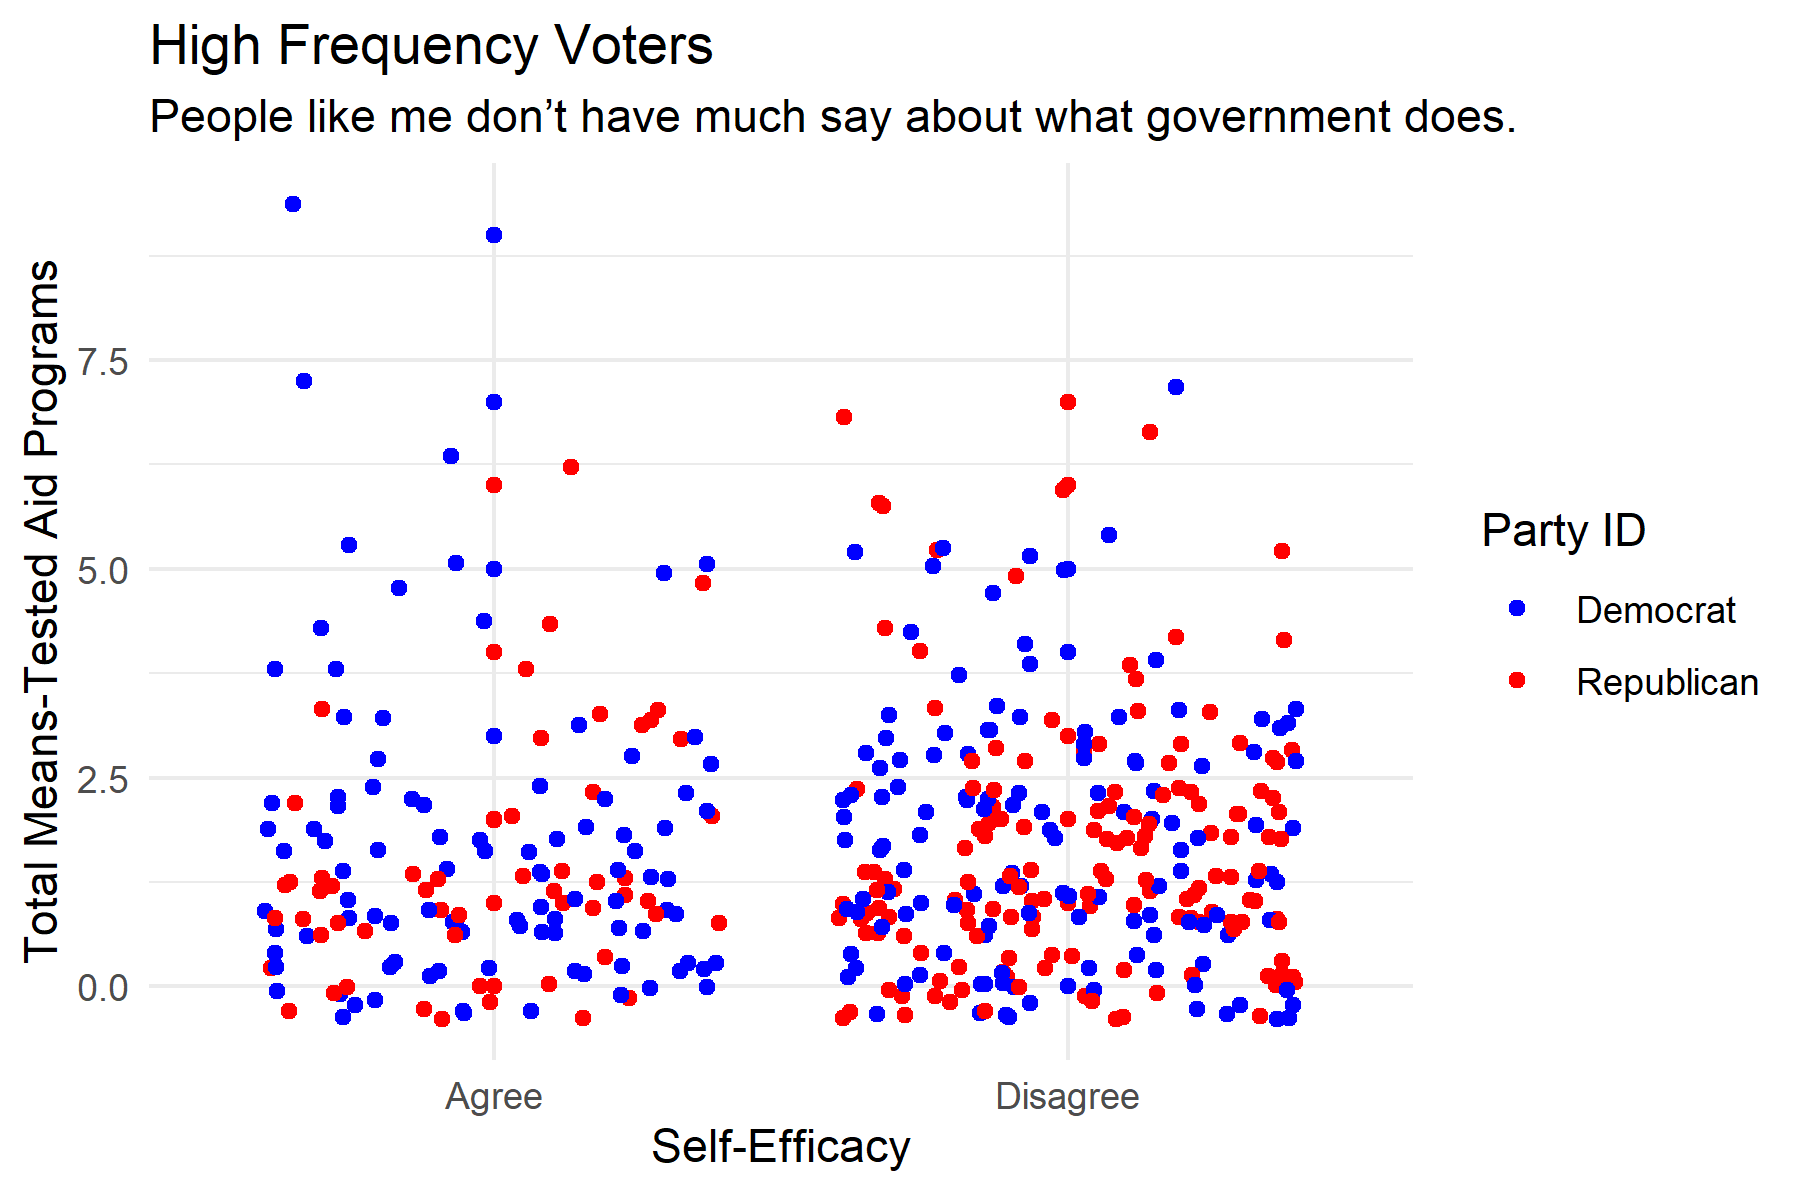
\includegraphics[scale=0.7]{Figs/scatter_means_efficacy_high.png} \centering
	\caption{}
	\label{}
\end{figure}


\begin{figure}[H]
	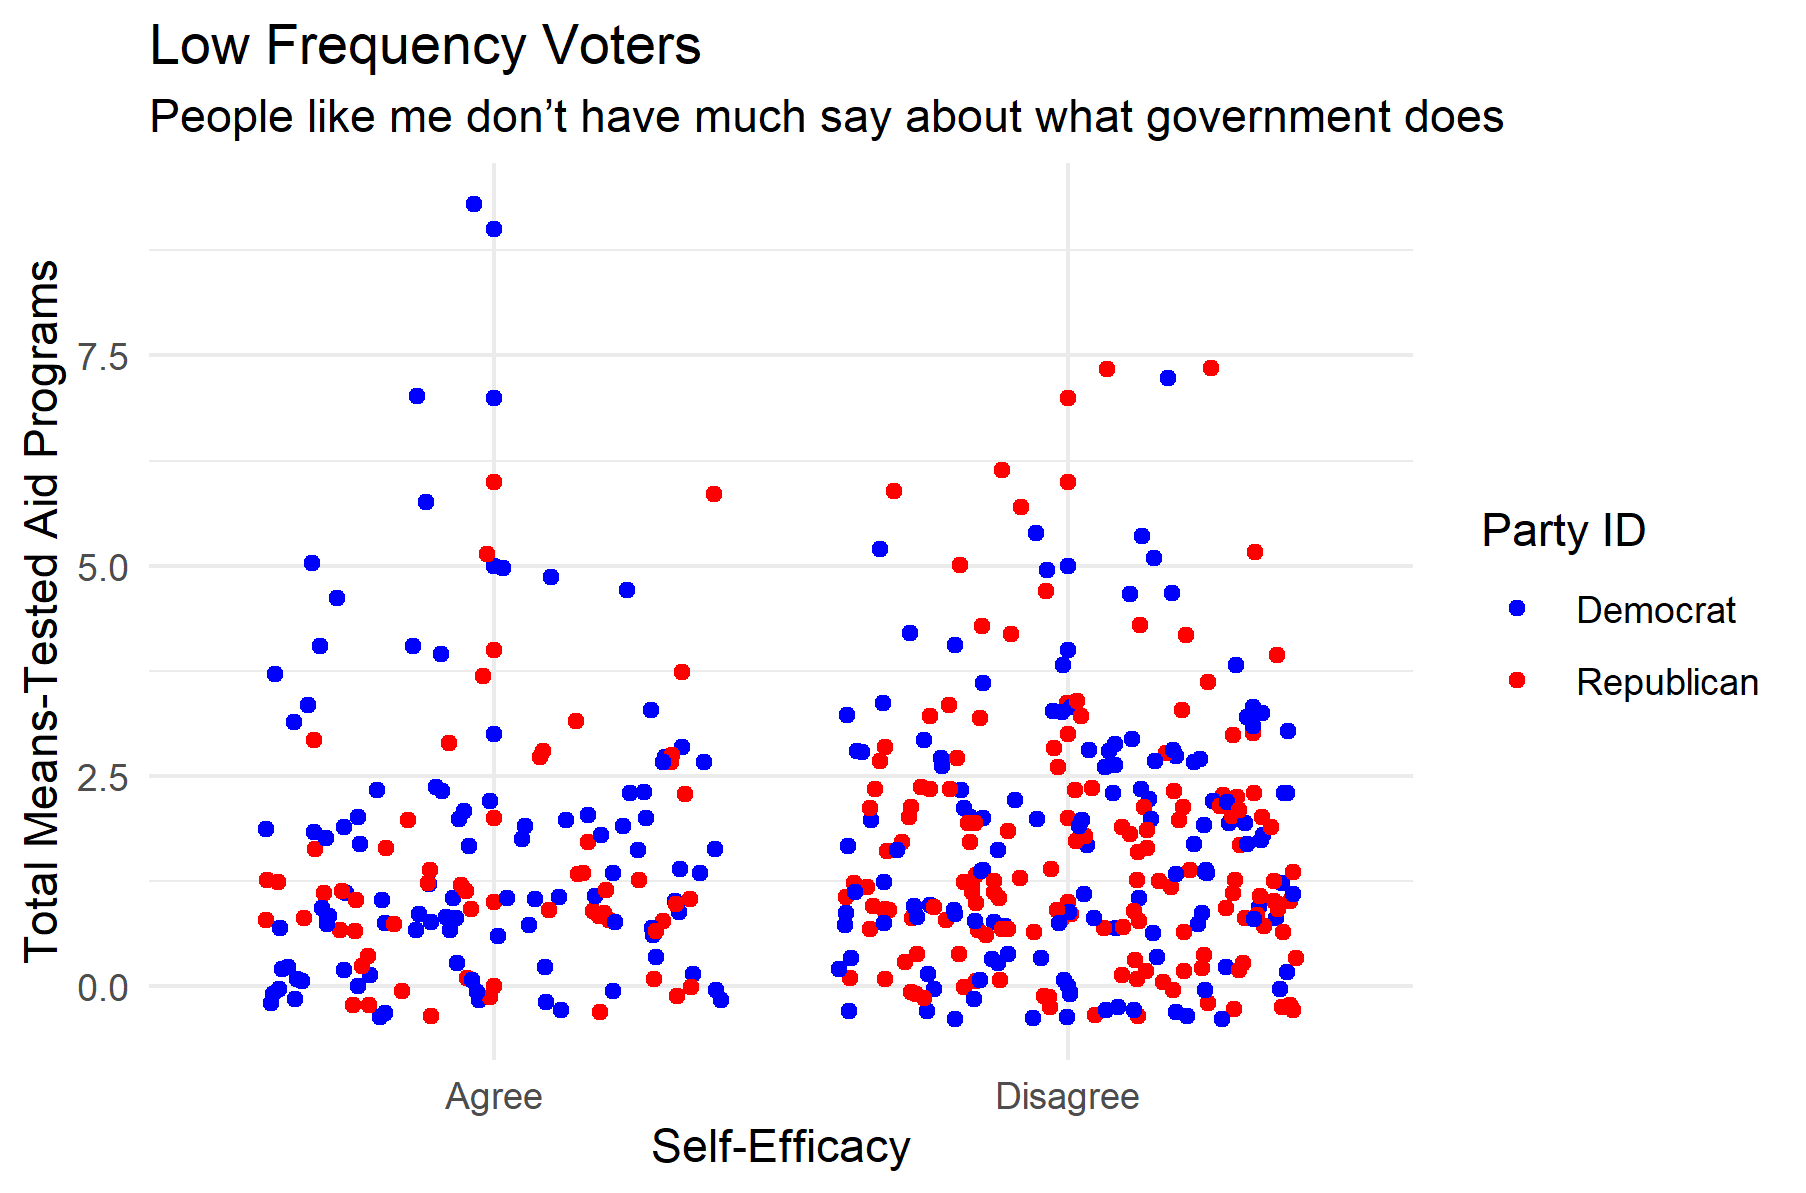
\includegraphics[scale=0.7]{Figs/scatter_means_efficacy_low.png} \centering
	\caption{}
	\label{}
\end{figure}

\begin{figure}[H]
	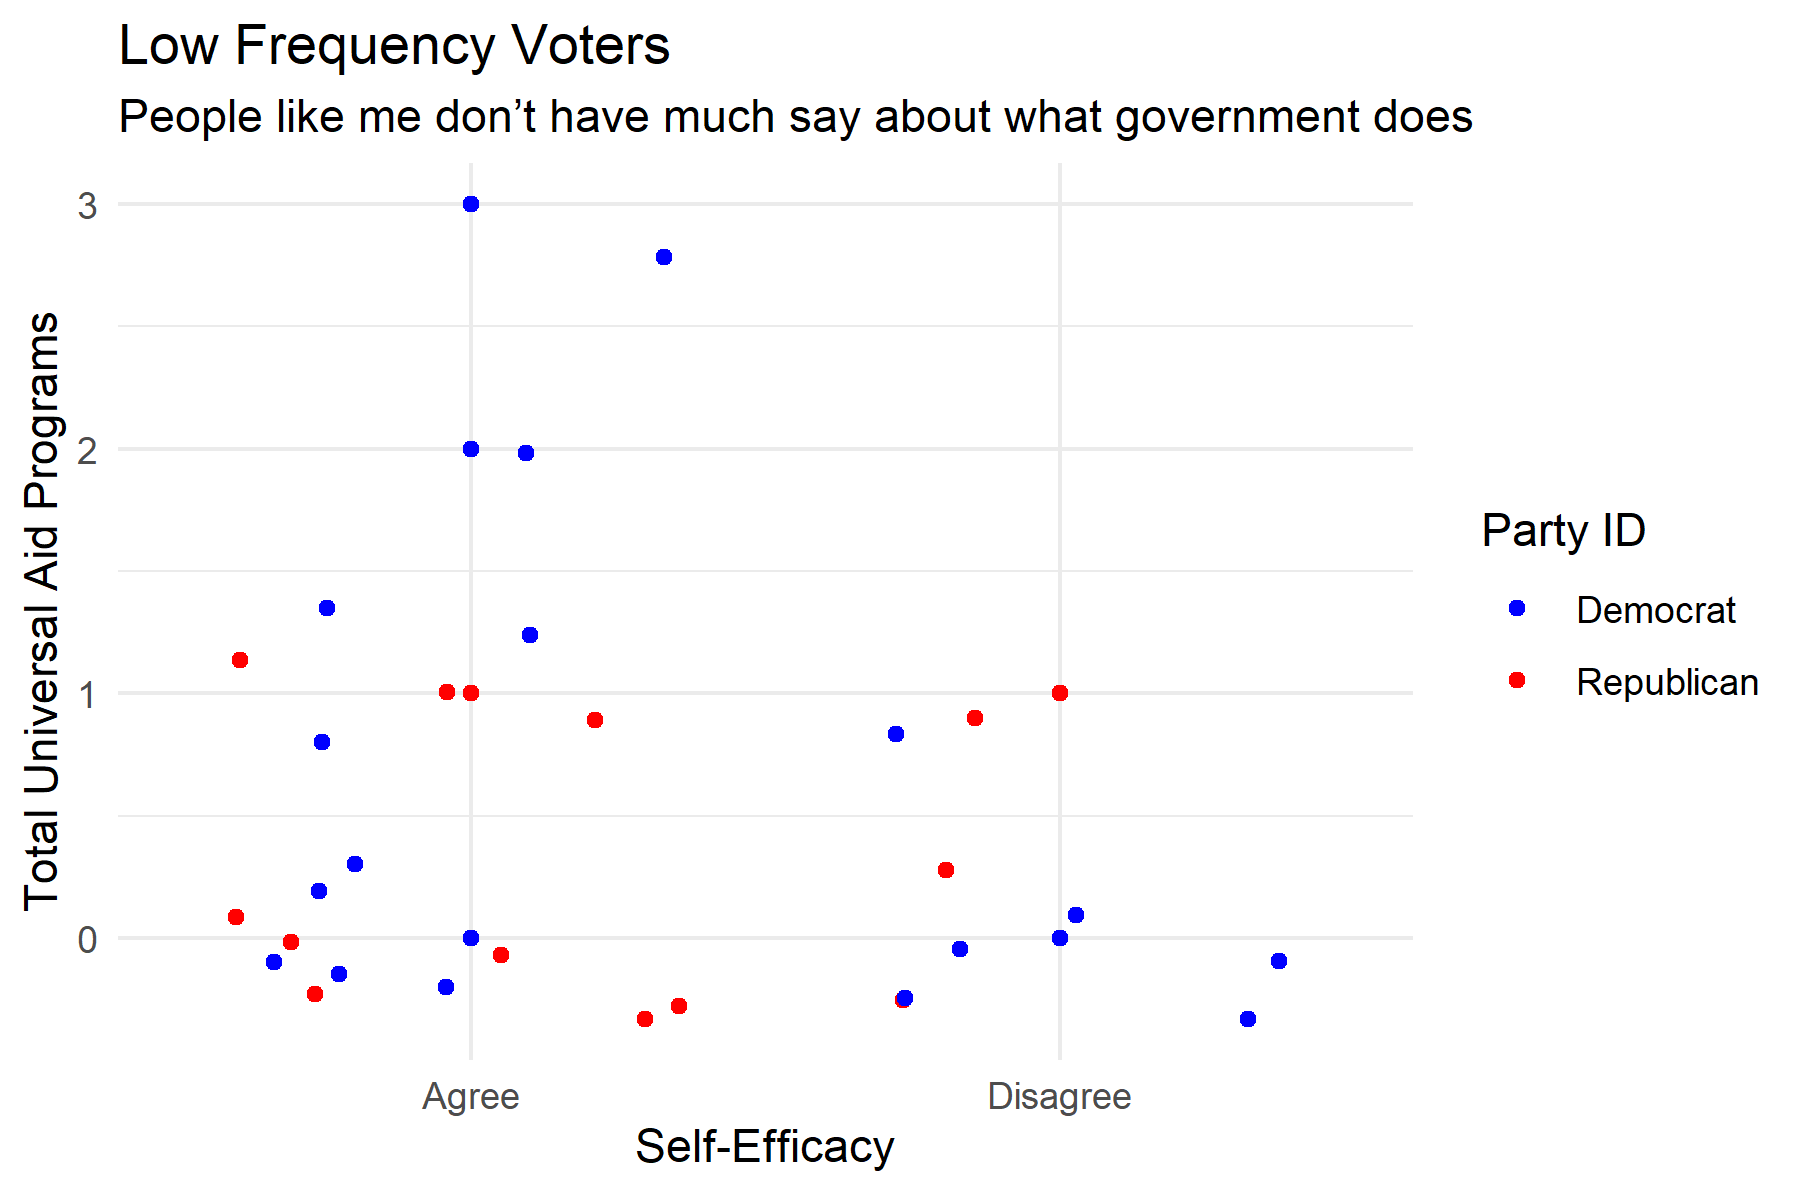
\includegraphics[scale=0.7]{Figs/scatter_uni_efficacy_low.png} \centering
	\caption{}
	\label{}
\end{figure}

\begin{figure}[H]
	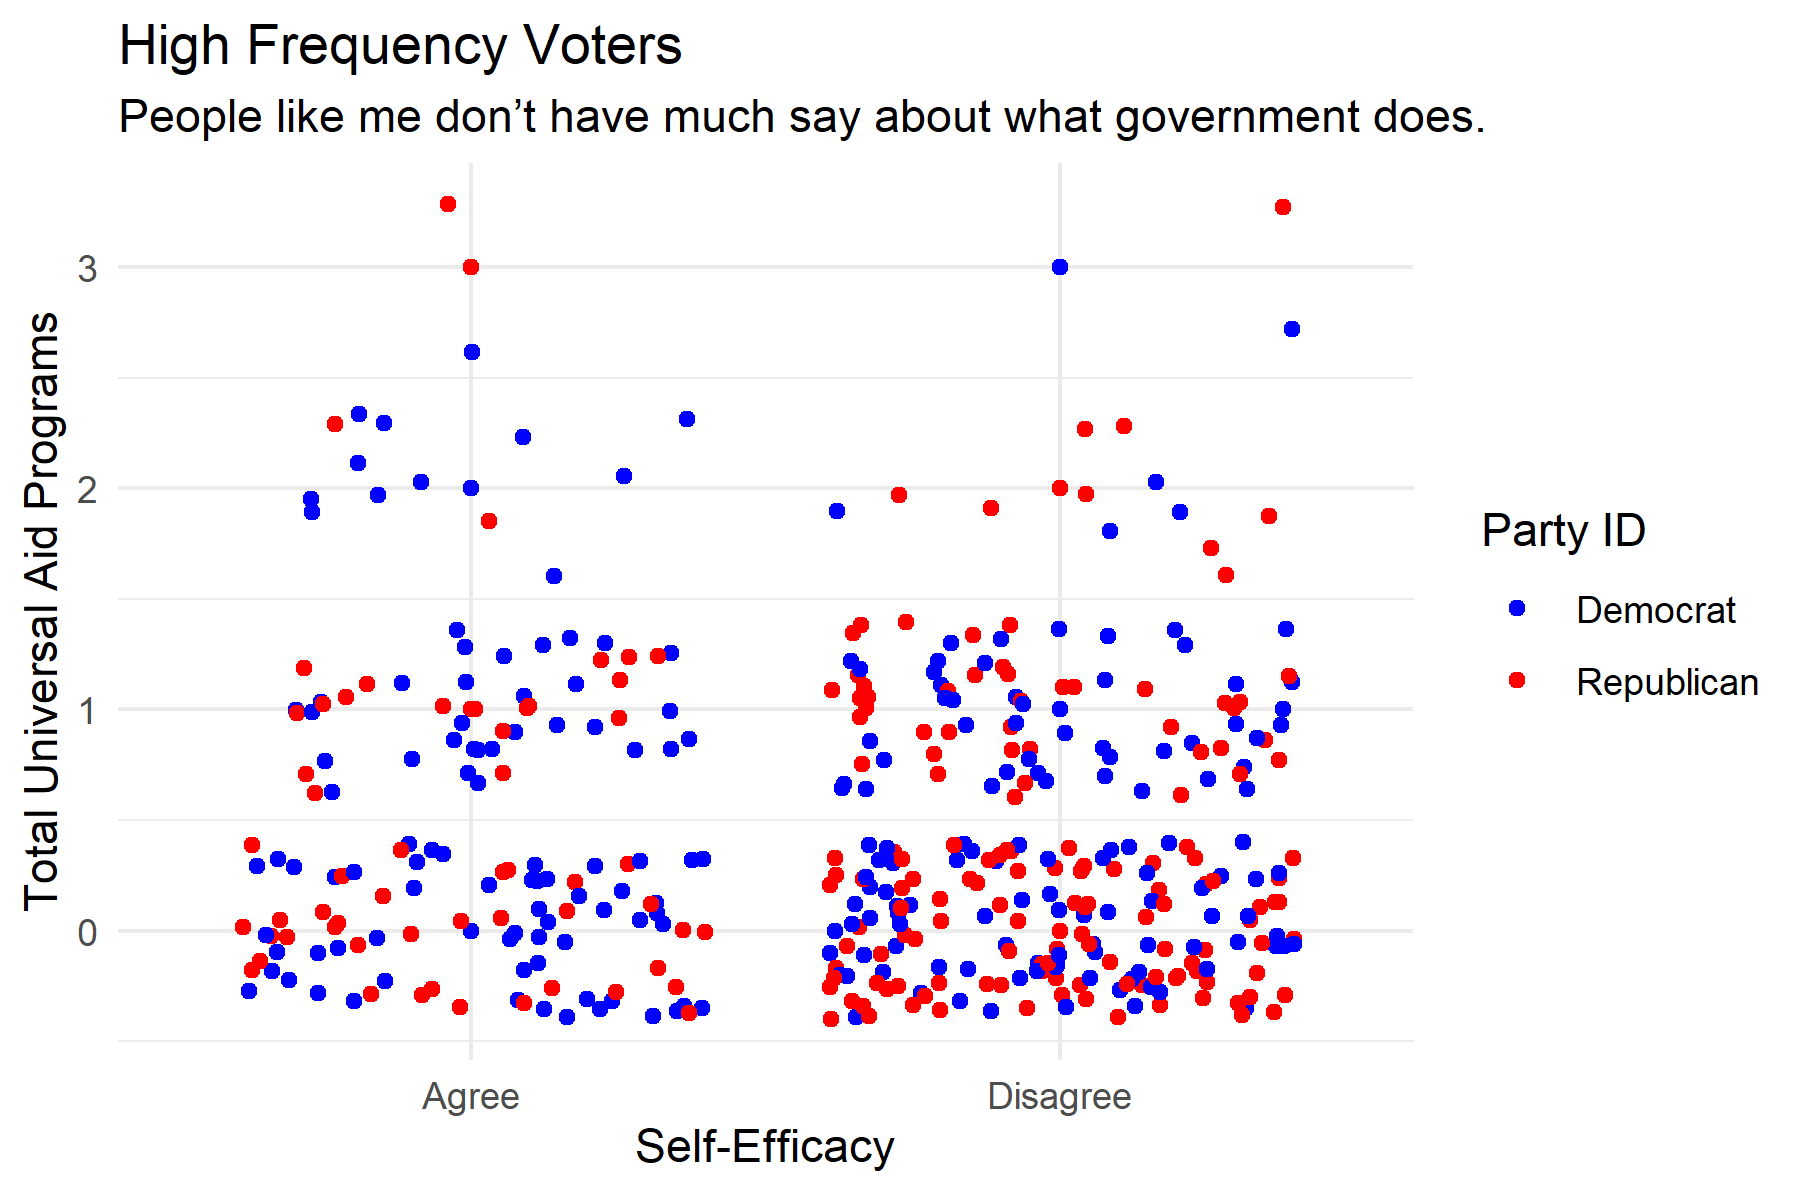
\includegraphics[scale=0.7]{Figs/scatter_uni_efficacy_high.png} \centering
	\caption{}
	\label{}
\end{figure}


\end{document}